\documentclass[12pt, a4paper]{article}

% --- PAKETLER ---
\usepackage[utf8]{inputenc}
\usepackage[T1]{fontenc}
\usepackage[turkish]{babel}
\usepackage[left=2.5cm, right=2.5cm, top=2.5cm, bottom=2.5cm]{geometry}
\usepackage{hyperref}
\usepackage{graphicx}
\usepackage{enumitem}
\usepackage{titlesec}
\usepackage{xcolor}
\usepackage{lmodern}
\usepackage{longtable}
\usepackage{array}
\usepackage{booktabs}
\usepackage{fancyhdr}
\usepackage{lastpage}
\usepackage{tabularx}
\usepackage{multirow}
\usepackage{float}
\usepackage{pdfpages}
\usepackage{pdflscape}
\usepackage{caption}
\usepackage{adjustbox}

% --- FONT AYARLARI ---
\renewcommand{\familydefault}{\rmdefault}

% --- RENKLER ---
\definecolor{darkblue}{RGB}{0, 51, 102}
\definecolor{lightgray}{RGB}{240, 240, 240}

% --- HYPERREF AYARLARI ---
\hypersetup{
    colorlinks=true,
    linkcolor=darkblue,
    urlcolor=darkblue,
    citecolor=darkblue,
    pdfauthor={Lagent},
    pdftitle={Yazılım Gereksinimleri Belirtimi (SRS)},
    pdfsubject={Çok Ajanlı Sözleşme İnceleme ve Müzakere Orkestratörü}
}

% --- BAŞLIK STİLLERİ ---
\titleformat{\section}
  {\Large\bfseries\color{darkblue}}
  {\thesection}{1em}{}
\titleformat{\subsection}
  {\large\bfseries\color{darkblue}}
  {\thesubsection}{1em}{}
\titleformat{\subsubsection}
  {\normalsize\bfseries\color{darkblue}}
  {\thesubsubsection}{1em}{}

% --- SAYFA BAŞLIK/ALTLIK ---
\pagestyle{fancy}
\fancyhf{}
\fancyhead[L]{\small\color{gray}Yazılım Gereksinimleri Belirtimi (SRS)}
\fancyhead[R]{\small\color{gray}Lagent}
\fancyfoot[C]{\small\color{gray}Sayfa \thepage\ / \pageref{LastPage}}
\renewcommand{\headrulewidth}{0.4pt}
\renewcommand{\footrulewidth}{0.4pt}

% --- LANDSCAPE SAYFALARI İÇİN BOŞ STİL ---
\fancypagestyle{landscapeempty}{%
  \fancyhf{}%
  \renewcommand{\headrulewidth}{0pt}%
  \renewcommand{\footrulewidth}{0pt}%
}

% --- LANDSCAPE ORTAMINDA OTOMATİK BAŞLIK/ALTLIK KALDIRMA ---
\usepackage{etoolbox}
\BeforeBeginEnvironment{landscape}{\pagestyle{landscapeempty}}
\AfterEndEnvironment{landscape}{\pagestyle{fancy}}

% --- BOŞLUK AYARLARI ---
\setlength{\parindent}{0pt}
\setlength{\parskip}{0.6em}

\begin{document}

% ============================================================
%  KAPAK SAYFASI (Cover Page)
% ============================================================
\begin{titlepage}
\centering
\vspace*{2cm}

{\Huge\bfseries\color{darkblue} Yazılım Gereksinimleri Belirtimi\\[0.3cm] (SRS)}

\vspace{1.5cm}

{\LARGE\bfseries Çok Ajanlı Sözleşme İnceleme ve\\[0.2cm] Müzakere Orkestratörü}

\vspace{0.5cm}

{\Large (Multi-Agent Legal Ops)}

\vspace{2cm}

\begin{tabular}{r l}
\textbf{Kurum:} & Gazi Üniversitesi \\[0.4cm]
\textbf{Grup İsmi:} & Lagent \\[0.4cm]
\textbf{Hazırlayanlar:} & Mustafa Emir Ceran -- 24118080702 \\
                        & Mert Ayrancı -- 24118080752 \\
                        & Osman Gazi Atalay -- 23118080703 \\[0.4cm]
\textbf{Tarih:} & 6 Nisan 2026 \\[0.4cm]
\textbf{Sürüm:} & 1.1 \\
\end{tabular}

\vfill


\end{titlepage}

% ============================================================
%  REVİZYON SAYFASI (Revisions Page)
% ============================================================
\newpage
\section*{Revizyon Geçmişi}
\addcontentsline{toc}{section}{Revizyon Geçmişi}

\begin{longtable}{|c|c|p{6cm}|c|}
\hline
\textbf{Sürüm} & \textbf{Tarih} & \textbf{Açıklama} & \textbf{Yazar} \\
\hline
\endfirsthead
\hline
\textbf{Sürüm} & \textbf{Tarih} & \textbf{Açıklama} & \textbf{Yazar} \\
\hline
\endhead
1.0 & 15.03.2026 & İlk sürüm oluşturuldu. & Lagent \\
\hline
1.1 & 06.04.2026 & SRS şablonuna uygun olarak bölüm yapısı güncellendi. Gerekli Durum ve Modlar, Uyarlama, Emniyet, Güvenlik ve Gizlilik, Ortam, Bilgisayar Kaynak, Yazılım Kalite Faktörleri, Tasarım Kısıtlamaları, Personel, Eğitim, Lojistik, Ambalajlama ve Öncelik/Kritiklik bölümleri eklendi. & Lagent \\
\hline
\end{longtable}

% ============================================================
%  İÇİNDEKİLER (Table of Contents)
% ============================================================
\newpage
\tableofcontents
\newpage

% ============================================================
%  1. GİRİŞ (INTRODUCTION)
% ============================================================
\section{GİRİŞ}

Bu Yazılım Gereksinimleri Belirtimi (SRS) dokümanı, Çok Ajanlı Sözleşme İnceleme ve Müzakere Orkestratörü (Multi-Agent Legal Ops) sisteminin işlevsel ve işlevsel olmayan gereksinimlerini kapsamlı biçimde tanımlamaktadır.

Dokümanın hedef kitlesi; yazılım geliştiriciler, test mühendisleri, proje yöneticileri, hukuki danışmanlar ve diğer paydaşlardır. Bu belge, sistemin ne yapması gerektiğini ortaya koyar; nasıl yapılacağına ilişkin tasarım kararları SDD (Software Design Document) kapsamında ele alınacaktır.

Günümüzde bireyler ve küçük-orta ölçekli işletmeler, kira sözleşmelerinden ticari anlaşmalara kadar geniş bir yelpazede hukuki metinlerle karşılaşmaktadır. Bu metinlerin doğru anlaşılması, risklerin zamanında tespit edilmesi ve gerektiğinde müzakere süreçlerinin yürütülmesi genellikle uzmanlık gerektiren, zaman alıcı ve maliyetli bir süreçtir. Mevcut durumda kullanıcılar çoğunlukla her sözleşme için ayrı avukat desteği almak zorunda kalmakta, bu da özellikle sıradan bireyler ve küçük işletmeler için erişilebilirlik sorunu yaratmaktadır.

Bu proje, söz konusu boşluğu doldurmak amacıyla çok ajanlı (multi-agent) bir yapay zeka asistanı geliştirmeyi hedeflemektedir. Sistem; sözleşme metinlerini otomatik olarak ayrıştıracak, madde bazında sınıflandıracak, kullanıcının belirlediği politikalara göre risk analizi yapacak, riskli maddeler için alternatif ifade önerileri sunacak ve tüm bu süreçleri bütünleşik bir onay akışı içinde yönetecektir.

Projenin temel motivasyonu, hukuki inceleme süreçlerinin demokratikleştirilmesi ve yapay zeka destekli otomasyon sayesinde hem zaman hem de maliyet tasarrufu sağlanmasıdır. Sistem, avukat desteğinin tamamen yerine geçmeyi değil; ön inceleme, risk tespiti ve müzakere hazırlığı aşamalarında kullanıcıya güvenilir bir asistanlık sunmayı amaçlamaktadır.

% ============================================================
%  1.1 ÜRÜN GENEL BAKIŞI (Product Overview)
% ============================================================
\subsection{Ürün Genel Bakışı}

\subsubsection{Ürün Perspektifi}
Çok Ajanlı Sözleşme İnceleme ve Müzakere Orkestratörü, bağımsız (stand-alone) bir web uygulaması olarak geliştirilecektir. Sistem herhangi bir mevcut kurumsal yazılımın parçası veya uzantısı değildir.

Sistem, birbiriyle koordineli çalışan birden fazla yapay zeka ajanından oluşan çok katmanlı bir mimari üzerine inşa edilecektir. Bu katmanlar genel hatlarıyla şöyledir:

\begin{enumerate}[leftmargin=2cm]
    \item \textbf{Doküman İşleme Katmanı:} Kullanıcının yüklediği sözleşme dosyalarının (PDF, DOCX vb.) düz metne dönüştürülmesi; taranmış belgeler için optik karakter tanıma (OCR) desteği sunulması.
    \item \textbf{Çok Ajanlı Yapay Zeka Katmanı:} Madde ayrıştırma, sınıflandırma, risk değerlendirme ve revizyon önerisi gibi görevlerin, her biri belirli bir sorumluluk alanına sahip bağımsız ajanlar tarafından yürütülmesi; bu ajanların bir orkestrasyon mekanizması aracılığıyla koordineli çalışması.
    \item \textbf{Bilgi Erişim Katmanı (RAG):} Kullanıcının tanımladığı politikalar (Playbook) ve referans madde havuzunun vektörel olarak indekslenmesi; analiz sırasında anlamsal benzerlik aramasıyla bağlam zenginleştirme yapılması.
    \item \textbf{Sunucu Tarafı API Katmanı:} İstemci uygulaması ile arka plan servisleri arasındaki iletişimi sağlayan, RESTful prensiplere uygun uygulama programlama arayüzü.
    \item \textbf{İstemci Katmanı:} Kullanıcıların sisteme eriştiği, sözleşme yükleyip analiz sonuçlarını incelediği, kararlarını verdiği modern web tabanlı arayüz.
    \item \textbf{Veri Yönetimi Katmanı:} İlişkisel veritabanı , vektör veritabanı , önbellek mekanizması ve nesne depolama  bileşenlerinin bütünleşik yönetimi.
\end{enumerate}

\subsubsection{Ürün İşlevleri}
Sistemin sunacağı başlıca işlevler aşağıda özetlenmiştir:

\begin{itemize}[leftmargin=2cm]
    \item \textbf{Sözleşme Yükleme ve Metin Dönüştürme:} Kullanıcıların farklı formatlardaki sözleşme dosyalarını sisteme yüklemesi; bu dosyaların otomatik olarak işlenebilir düz metne dönüştürülmesi.
    \item \textbf{Madde Bazlı Ayrıştırma:} Sözleşme metninin yapısal olarak ayrı maddelere bölünmesi ve her maddenin bağımsız bir birim olarak ele alınması.
    \item \textbf{Otomatik Sınıflandırma:} Ayrıştırılan her maddenin, önceden tanımlanmış hukuki kategorilere (gizlilik, tazminat, fesih, fikri mülkiyet, sorumluluk sınırlandırma, uyuşmazlık çözümü, ödeme koşulları vb.) yapay zeka destekli olarak atanması.
    \item \textbf{Politika Uyumluluk Kontrolü:} Her maddenin, kullanıcının tanımladığı Playbook kurallarına göre uyumluluk açısından değerlendirilmesi; eksik veya çelişkili hükümlerin otomatik tespit edilmesi.
    \item \textbf{Risk Değerlendirmesi:} Maddelerin ticari ve hukuki boyutlarıyla birlikte çok seviyeli bir risk skalasında (düşük, orta, yüksek) derecelendirilmesi.
    \item \textbf{Revizyon Önerisi Üretimi:} Riskli bulunan maddeler için, kullanıcı politikaları ve referans madde havuzu temelinde alternatif ifade önerilerinin otomatik olarak üretilmesi.
    \item \textbf{Karşılaştırmalı Görünüm (Redline):} Orijinal madde metni ile önerilen revizyon metninin, ekleme ve silme farklarının görsel olarak vurgulandığı karşılaştırmalı bir biçimde sunulması.
    \item \textbf{Onay Akışı Yönetimi:} Her madde için ayrı ayrı onay, red veya yeniden revize kararı verilebilmesi; bu kararların durum geçişleriyle (taslak, incelemede, onaylandı, reddedildi) izlenebilmesi.
    \item \textbf{Denetim İzi (Audit Trail):} Kullanıcıların verdiği tüm kararların, yorumların ve işlem zaman damgalarının kayıt altına alınması.
    \item \textbf{Raporlama ve Dışa Aktarım:} İnceleme sonuçlarının özet ve detaylı rapor olarak görüntülenmesi; raporların ve revize edilmiş sözleşme taslağının dosya olarak indirilebilmesi.
    \item \textbf{Playbook Yönetimi:} Kullanıcıların kendi sözleşme politikalarını (kabul edilebilir ifadeler, reddedilecek ifadeler, eşik değerler) tanımlayabilmesi, düzenleyebilmesi ve bu kuralların analiz sürecine yansıtılması.
\end{itemize}

\subsubsection{Kullanıcı Sınıfları ve Özellikleri}
Sistemin hedef kullanıcı kitleleri aşağıdaki gibi sınıflandırılmaktadır:

\begin{longtable}{|p{3cm}|p{5.5cm}|p{5cm}|}
\hline
\textbf{Kullanıcı Tipi} & \textbf{Profil} & \textbf{Teknik Yeterlilik} \\
\hline
Bireysel Kullanıcı & Kira, iş veya hizmet sözleşmelerini inceleyen bireyler. Hukuki terminolojiye aşinalıkları sınırlıdır. & Temel bilgisayar ve internet kullanımı. Hukuki ön bilgi gerektirmez. \\
\hline
KOBİ Yöneticisi & Ticari sözleşmeleri, tedarikçi anlaşmalarını ve ortaklık protokollerini inceleyen küçük-orta ölçekli işletme sahipleri veya yöneticileri. & Orta düzey bilgisayar kullanımı. Temel ticari sözleşme bilgisi. \\
\hline
Hukuk Danışmanı & Sözleşme inceleme sürecini hızlandırmak, ön tarama ve risk analizini otomatikleştirmek isteyen avukatlar ve hukuk müşavirleri. & İleri düzey hukuki bilgi, orta düzey teknik yeterlilik. \\
\hline
Sistem Yöneticisi & Platformun kurulumu, yapılandırması, kullanıcı yönetimi ve bakım süreçlerini yürüten teknik personel. & İleri düzey teknik yeterlilik. Sunucu yönetimi ve veritabanı bilgisi. \\
\hline
\end{longtable}

\subsubsection{Çalışma Ortamı}
Sistem bir web uygulaması olarak çalışacaktır. Kullanıcılar, modern bir web tarayıcısı aracılığıyla herhangi bir ek yazılım kurulumu gerektirmeden sisteme erişebilecektir. Sunucu tarafı bileşenleri konteynerize edilerek farklı altyapı ortamlarında çalıştırılabilecektir.

\subsubsection{Tasarım ve Uygulama Kısıtları}
\begin{itemize}[leftmargin=2cm]
    \item Sistem, doğal dil işleme ve metin üretimi görevlerinde harici bir büyük dil modeli (LLM) servisine bağımlıdır. Bu servisin erişilebilirliği ve yanıt kalitesi, sistem performansını doğrudan etkiler.
    \item Optik karakter tanıma (OCR) doğruluğu, yüklenen taranmış dokümanların görüntü kalitesine bağlıdır; düşük çözünürlüklü veya bozuk taramalar hatalı metin çıktısına yol açabilir.
    \item Sistem, hukuki tavsiye niteliği taşımaz ve bir avukatın yerini almayı hedeflemez. Nihai karar ve sorumluluk her zaman kullanıcıya aittir.
    \item İlk sürümde yalnızca Türkçe sözleşme metinleri desteklenecektir.
    \item Yüksek risk seviyesindeki maddelerde otomatik onay mekanizması uygulanmayacak; bu maddelerde insan onayı zorunlu olacaktır.
    \item Yapay zeka modelinin ürettiği tüm çıktılar (sınıflandırma, risk skoru, revizyon önerisi), deterministik olmayan doğası gereği yanlış pozitif veya yanlış negatif sonuçlar içerebilir; bu nedenle çapraz doğrulama mekanizmaları uygulanacaktır.
\end{itemize}

\subsubsection{Varsayımlar ve Bağımlılıklar}
\begin{itemize}[leftmargin=2cm]
    \item Kullanıcıların güncel bir web tarayıcısına ve stabil bir internet bağlantısına sahip olduğu varsayılmaktadır.
    \item Harici dil modeli servisinin kesintisiz ve kabul edilebilir gecikme süreleriyle erişilebilir olduğu varsayılmaktadır.
    \item Kullanıcıların sisteme yükleyeceği sözleşme dosyalarının makine tarafından okunabilir kalitede olduğu varsayılmaktadır.
    \item Sunucu tarafı altyapı bileşenlerinin (veritabanı, önbellek, dosya depolama) konteyner ortamında çalıştırılacağı varsayılmaktadır.
    \item Kullanıcıların Playbook oluştururken temel sözleşme terminolojisine aşina olduğu varsayılmaktadır, sistem yorumlayıcı katman içerdiği için Playbook girdisi kapsayıcı ve konuyla alakalı olmalıdır.
\end{itemize}

% ============================================================
%  2. GEREKSİNİMLER
% ============================================================
\newpage
\section{GEREKSİNİMLER}

% ============================================================
%  2.1 GEREKLİ DURUM VE MODLAR
% ============================================================
\subsection{Gerekli Durum ve Modlar}

Sistem aşağıdaki çalışma durumlarına sahip olacaktır:

\begin{description}[leftmargin=2cm, style=nextline]
    \item[Boşta (Idle)]
    Kullanıcı oturum açmış ancak herhangi bir analiz işlemi başlatmamıştır. Sistem, yeni görev bekleme durumundadır; kullanıcı dashboard'u görüntüleyebilir, sözleşme listesine göz atabilir veya Playbook yönetimi yapabilir.

    \item[Aktif -- Analiz İşlemi]
    Kullanıcı bir sözleşme yüklemiş ve otomatik analiz süreci başlamıştır. Bu durumda ayrıştırma, sınıflandırma, risk değerlendirme ve revizyon önerisi ajanları sıralı/paralel olarak çalışmaktadır. Kullanıcıya gerçek zamanlı ilerleme bildirimi gönderilir.

    \item[Aktif -- İnceleme ve Karar]
    Analiz tamamlanmış, kullanıcı madde bazlı sonuçları incelemekte ve onay/red kararlarını vermektedir. Bu modda yapay zeka ajanları pasiftir; kullanıcı etkileşimi ön plandadır.

    \item[Bozulmuş (Degraded)]
    Harici dil modeli (LLM) servisi veya bir altyapı bileşeni (veritabanı, önbellek vb.) erişilemez durumdadır. Sistem, daha önce tamamlanmış analiz sonuçlarına erişimi sürdürür ancak yeni analiz başlatılamaz. Kullanıcıya uygun hata mesajı gösterilir.

    \item[Bakım (Maintenance)]
    Planlı bakım süresinde sistem geçici olarak kullanıma kapatılır. Kullanıcılara bakım bildirimi gösterilir.
\end{description}

Her gereksinim, ilgili durum ve modlarla ilişkilidir. Fonksiyonel gereksinimler ağırlıklı olarak \textit{Aktif -- Analiz İşlemi} ve \textit{Aktif -- İnceleme ve Karar} durumlarıyla; güvenilirlik ve hata yönetimi gereksinimleri \textit{Bozulmuş} durumuyla ilişkilidir.

% ============================================================
%  2.2 YKE FONKSİYONEL GEREKSİNİMLERİ
% ============================================================
\subsection{YKE Fonksiyonel Gereksinimleri}

Bu bölüm, sistemin her bir fonksiyonel alanı ile ilişkili gereksinimleri ayrıntılandırmak üzere alt paragraflara bölünmüştür.

\subsubsection{Kullanıcı Kayıt ve Kimlik Doğrulama}
\begin{enumerate}[leftmargin=2cm]
    \item Sistem, kullanıcıların e-posta adresi ve şifre ile yeni hesap oluşturmasına izin verecektir.
    \item Sistem, token tabanlı bir kimlik doğrulama mekanizması kullanacaktır.
    \item Başarısız giriş denemelerinde kullanıcıya anlaşılır hata mesajları gösterilecektir.
\end{enumerate}

\subsubsection{Sözleşme Yükleme ve Doküman İşleme}
\begin{enumerate}[leftmargin=2cm]
    \item Sistem, en yaygın doküman formatlarını (PDF, DOCX) kabul edecektir.
    \item Yüklenen dosya boyutu, yapılandırılabilir bir üst limite (varsayılan 10~MB) tabi olacaktır.
    \item Sistem, yüklenen dokümanları otomatik olarak düz metne dönüştürecektir.
    \item Taranmış (görüntü tabanlı) belgelerde metin çıkarımı için optik karakter tanıma (OCR) uygulanacaktır.
    \item Dönüştürme işlemi başarısız olduğunda kullanıcıya nedenini açıklayan anlamlı bir hata mesajı gösterilecektir.
    \item Yüklenen orijinal dosyalar, nesne depolama servisi üzerinde güvenli biçimde saklanacaktır.
\end{enumerate}

\subsubsection{Madde Ayrıştırma ve Sınıflandırma}
\begin{enumerate}[leftmargin=2cm]
    \item Ayrıştırma ajanı (Clause Agent), dönüştürülmüş metni sözleşme maddelerine bölecektir.
    \item Her madde; gizlilik, tazminat, fesih, fikri mülkiyet, sorumluluk sınırlandırma, uyuşmazlık çözümü, ödeme koşulları ve genel hükümler gibi önceden tanımlanmış kategorilere sınıflandırılacaktır.
    \item Sınıflandırma sonuçları, yapılandırılmış veri formatında döndürülecektir.
    \item Sistem, her madde için sınıflandırma güven skorunu (confidence score) hesaplayacaktır.
    \item Güven skoru belirlenen eşiğin altında kalan maddeler ``Belirsiz'' olarak işaretlenecek ve kullanıcının manuel doğrulamasına sunulacaktır.
    \item 10 sayfalık standart bir sözleşmenin maddelere ayrıştırılması ve sınıflandırılması 120 saniye içinde tamamlanacaktır. (Yanıt süresi LLM servisine göre değişkenlik gösterebilir.)
\end{enumerate}

\subsubsection{Politika Kontrolü ve Risk Değerlendirmesi}
\begin{enumerate}[leftmargin=2cm]
    \item Risk değerlendirme ajanı (Risk Agent), sınıflandırılmış maddeleri kullanıcının Playbook'undaki kurallarla karşılaştıracaktır.
    \item Karşılaştırma işlemi, anlamsal benzerlik araması (RAG altyapısı) kullanılarak gerçekleştirilecektir.
    \item Her maddeye düşük, orta ve yüksek olmak üzere üç seviyeli bir risk derecesi atanacaktır.
    \item Risk değerlendirmesi, hem ticari hem de hukuki boyutları kapsayan çok boyutlu bir rubriğe dayandırılacaktır.
    \item Playbook'ta tanımlanan ancak sözleşmede yer almayan hükümler otomatik olarak tespit edilecek ve raporlanacaktır.
    \item Yapay zeka modelinin ürettiği risk değerlendirmeleri, deterministik kural mekanizmalarıyla çapraz doğrulanacaktır.
    \item Risk değerlendirme sonuçlarında her madde için riskin gerekçesi açıklama olarak sunulacaktır.
    \item Bir sözleşmenin tüm maddeleri için risk değerlendirmesi 120 saniye içinde tamamlanacaktır. (Yanıt süresi LLM servisine göre değişkenlik gösterebilir.)
\end{enumerate}

\subsubsection{Revizyon Önerisi ve Karşılaştırmalı Görünüm}
\begin{enumerate}[leftmargin=2cm]
    \item Sistem, yüksek ve kritik risk seviyesindeki maddeler için otomatik olarak alternatif ifade önerileri üretecektir.
    \item Öneri üretiminde kullanıcı Playbook'u bağlam olarak kullanılacaktır.
    \item Orijinal ve önerilen metinler arasındaki farklar, karşılaştırmalı (redline/diff) formatta görüntülenecektir.
    \item Kullanıcı, sistem tarafından önerilen revizyon metnini doğrudan arayüz üzerinden düzenleyebilecektir.
    \item Gerektiğinde revize edilmiş sözleşmenin doküman formatında dışa aktarılması sağlanacaktır.
\end{enumerate}

\subsubsection{Onay Akışı}
\begin{enumerate}[leftmargin=2cm]
    \item Onay akışı, durum makinesi mantığıyla yönetilecektir. Temel durum geçişleri: \textit{Taslak Oluşturuldu $\rightarrow$ İncelemede $\rightarrow$ Onay Bekliyor $\rightarrow$ Onaylandı / Reddedildi}.
    \item Her madde için bağımsız olarak onay, red veya yeniden revize kararı verilebilecektir.
    \item Yüksek risk seviyesindeki maddelerde otomatik onay yapılmayacak; insan onayı zorunlu olacaktır.
    \item Tüm onay ve red kararları; karar veren kullanıcı bilgisi, zaman damgası ve varsa yorum ile birlikte denetim izi (audit trail) olarak kaydedilecektir.
    \item Reddedilen veya revize edilen maddeler, güncellenmiş öneriyle birlikte yeniden değerlendirme döngüsüne alınabilecektir.
\end{enumerate}

\subsubsection{Raporlama}
\begin{enumerate}[leftmargin=2cm]
    \item Sistem, sözleşme inceleme sonuçlarını özet rapor olarak gösterecektir. Özet raporda toplam madde sayısı, risk seviyesi dağılımı ve karar durumları yer alacaktır.
    \item Detaylı rapor, her madde için kategori, risk seviyesi, risk gerekçesi, verilen karar ve kullanıcı yorumu bilgilerini içerecektir.
    \item Raporlar, PDF ve DOCX formatlarında indirilebilecektir.
\end{enumerate}

\subsubsection{Playbook Yönetimi}
\begin{enumerate}[leftmargin=2cm]
    \item Kullanıcı, kendi sözleşme politikalarını (Playbook) oluşturabilecek, düzenleyebilecek ve silebilecektir.
    \item Playbook kuralları; kabul edilebilir ifadeler, reddedilecek ifadeler, zorunlu olması gereken hükümler ve sayısal eşik değerler olarak yapılandırılabilecektir.
    \item Playbook güncellendiğinde, ilgili vektörel indeksler otomatik olarak yenilenecektir.
    \item Kullanıcı, birden fazla Playbook tanımlayabilecek ve sözleşme analizinde hangi Playbook'un kullanılacağını seçebilecektir.
    \item Sistem, varsayılan bir Playbook şablonu sunacaktır; kullanıcılar bu şablonu temel alarak kendi kurallarını oluşturabilecektir.
\end{enumerate}

% ============================================================
%  2.3 YKE DIŞ ARAYÜZ GEREKSİNİMLERİ
% ============================================================
\subsection{YKE Dış Arayüz Gereksinimleri}

Bu bölüm, sistemin harici arayüzleri (kullanıcılar, harici servisler ve diğer sistemlerle veri bölüşme, sağlama veya değiştirme gerektiren ilişkiler) için gereksinimleri belirtir.

\subsubsection{Arayüz Tanımlaması ve Diyagramları}

Sistemin harici arayüzleri aşağıda tanımlanmaktadır:

\begin{longtable}{|p{3.5cm}|p{3cm}|p{7cm}|}
\hline
\textbf{Arayüz Elemanı} & \textbf{Tip} & \textbf{Açıklama} \\
\hline
\endfirsthead
\hline
\textbf{Arayüz Elemanı} & \textbf{Tip} & \textbf{Açıklama} \\
\hline
\endhead
Web Kullanıcı Arayüzü & Kullanıcı--Sistem & Kullanıcıların tüm sistem işlevlerine eriştiği web tabanlı ön yüz arayüzü. \\
\hline
LLM API Arayüzü & Sistem--Sistem & Yapay zeka görevleri (sınıflandırma, risk analizi, revizyon) için harici büyük dil modeli servisine yapılan API çağrıları. \\
\hline
RESTful API & İstemci--Sunucu & İstemci uygulaması ile sunucu tarafı servisleri arasındaki yapılandırılmış veri iletişimi. \\
\hline
WebSocket Arayüzü & Sunucu--İstemci & Uzun süren işlemlerde gerçek zamanlı ilerleme bildirimi. \\
\hline
\end{longtable}

% --- 2.3.2 Kullanıcı Arayüzü ---
\subsubsection{Kullanıcı Arayüzü (UI-01)}

Sistemin kullanıcı arayüzü, web tabanlı bir dashboard üzerinden sunulacaktır. Arayüz tasarımında sadelik, tutarlılık ve kullanıcı dostu deneyim ön planda tutulacaktır. Aşağıda sistemin temel ekranları ve beklenen davranışları açıklanmaktadır.

\begin{description}[leftmargin=2cm, style=nextline]
    \item[Giriş ve Kimlik Doğrulama Ekranı]
    Kullanıcıların e-posta adresi ve şifre ile sisteme giriş yapabileceği ekrandır. Yeni kayıt oluşturma işlevini de içerecektir. Başarısız giriş denemelerinde kullanıcıya anlaşılır hata mesajları gösterilecektir.

    \item[Ana Kontrol Paneli (Dashboard)]
    Kullanıcının sisteme giriş yaptıktan sonra karşılaştığı ana ekrandır. Bu ekranda; daha önce yüklenen sözleşmelerin listesi, her sözleşmenin mevcut durumu (inceleniyor, tamamlandı, onay bekliyor gibi), genel risk dağılımı istatistikleri ve hızlı erişim kısayolları yer alacaktır.

    \item[Sözleşme Yükleme Ekranı]
    Kullanıcının yeni bir sözleşme dosyası yükleyebildiği ekrandır. Sürükle-bırak ve dosya seçici yöntemlerini destekleyecektir. Kabul edilen dosya formatları ve maksimum dosya boyutu konusunda kullanıcıya önceden bilgi verilecektir. Dosya format ve boyut doğrulaması istemci tarafında anlık olarak yapılacaktır.

    \item[Sözleşme İnceleme ve Analiz Ekranı]
    İncelenen sözleşmenin detaylı görünümüdür. Sol panelde ayrıştırılmış sözleşme maddelerinin listesi; sağ panelde seçili maddenin tam metni, atandığı kategori, risk seviyesi, politika uyumluluk durumu ve varsa revizyon önerisi gösterilecektir. Maddeler risk seviyelerine göre renk kodlaması ile görsel olarak ayrıştırılacaktır (örn. düşük risk için yeşil, kritik risk için kırmızı tonları).

    \item[Karşılaştırmalı Görünüm (Redline) Ekranı]
    Orijinal madde metni ile önerilen revizyon metninin yan yana veya satır içi karşılaştırmalı biçimde gösterildiği ekrandır. Metne eklenen kısımlar ve silinen kısımlar farklı renklerle vurgulanarak kullanıcının değişiklikleri hızlıca kavraması sağlanacaktır.

    \item[Onay Akışı Paneli]
    Her sözleşme maddesi için karar verme ekranıdır. Kullanıcı, her madde için onayla, reddet veya yeniden revize et seçeneklerinden birini işaretleyebilecektir. Her karara açıklayıcı yorum eklenebilir. Daha önce verilmiş kararların geçmişi kronolojik olarak listelenecektir. İsteğe bağlı olarak toplu karar verme (birden fazla maddeyi aynı anda onaylama/reddetme) desteği sunulacaktır.

    \item[Rapor ve Dışa Aktarım Ekranı]
    İnceleme sürecinin sonuçlarının özet ve detaylı rapor olarak görüntülendiği ekrandır. Raporlar; toplam madde sayısı, risk seviyesi dağılımı, verilen kararların özeti ve madde bazlı detayları içerecektir. Kullanıcı, raporları ve revize edilmiş sözleşme taslağını dosya olarak indirebilecektir.

    \item[Playbook Yönetim Ekranı]
    Kullanıcının kendi sözleşme politikalarını oluşturduğu ve yönettiği ekrandır. Kabul edilebilir madde ifadeleri, reddedilmesi gereken hükümler ve eşik değerler bu ekran üzerinden tanımlanacaktır. Mevcut Playbook kuralları listelenebilecektir, düzenlenebilecektir ve silinebilecektir.
\end{description}

\textbf{Genel Kullanıcı Arayüzü Gereksinimleri:}
\begin{itemize}[leftmargin=2cm]
    \item Arayüz responsive tasarıma sahip olacak ve masaüstü tarayıcılarda (minimum 1280$\times$720 piksel çözünürlük) görüntüleme sağlayacaktır.
    \item Tüm kullanıcı işlemleri için anlık görsel geri bildirim sağlanacaktır (yükleniyor göstergesi, başarı bildirimi, hata mesajı vb.).
    \item Sözleşme analizi, risk skorlama sırasında kullanıcıya ilerleme durumu gerçek zamanlı olarak bildirilecektir.
    \item Arayüz dili Türkçe olacaktır.
\end{itemize}

\textbf{Veri Elemanları:}

Kullanıcı arayüzü üzerinden sağlanacak ve görüntülenecek temel veri elemanları aşağıda belirtilmiştir:

\begin{itemize}[leftmargin=2cm]
    \item \textbf{Sözleşme dosyası (girdi):} PDF veya DOCX formatında, maksimum 10~MB boyutunda dosya.
    \item \textbf{Madde listesi (çıktı):} Madde sıra numarası (tam sayı), madde metni (metin), kategori (metin), risk seviyesi (düşük/orta/yüksek), güven skoru (0--1 arası ondalık).
    \item \textbf{Revizyon önerisi (çıktı):} Orijinal metin (metin), önerilen metin (metin), fark görünümü (HTML formatında).
    \item \textbf{Karar bilgisi (girdi):} Karar türü (onaylandı/reddedildi/revize), kullanıcı yorumu (metin, isteğe bağlı).
    \item \textbf{Rapor (çıktı):} Özet rapor verileri (sayısal istatistikler), detaylı rapor (madde bazlı tablo formatında).
\end{itemize}

% --- 2.3.3 Yazılım Arayüzleri ---
\subsubsection{LLM Servisi Arayüzü (SW-01)}

Sistem, madde sınıflandırma, risk değerlendirme, revizyon önerisi üretimi ve doğal dil anlama görevlerini yerine getirmek için harici bir büyük dil modeli servisine bağlanacaktır. İletişim, standart API çağrılarıyla sağlanacak ve veri alışverişinde JSON formatı kullanılacaktır.

\begin{itemize}[leftmargin=2cm]
    \item \textbf{Arayüz tipi:} Gerçek zamanlı veri transferi (istek/yanıt).
    \item \textbf{Öncelik:} Yüksek -- analiz işlemlerinin temel bağımlılığıdır.
    \item \textbf{Veri formatı:} JSON (UTF-8 kodlamalı metin).
    \item \textbf{Güvenlik:} API anahtarı ile kimlik doğrulama; HTTPS üzerinden şifrelenmiş iletişim.
\end{itemize}

\subsubsection{Veritabanı Arayüzü (SW-02)}

Kullanıcı hesapları, sözleşme meta verileri, ayrıştırılmış madde kayıtları, risk değerlendirme sonuçları, onay kararları ve denetim izi (audit trail) verilerinin kalıcı olarak saklanması için ilişkisel bir veritabanı kullanılacaktır.

\subsubsection{Vektör Arama Arayüzü (SW-03)}

Sözleşme maddelerinin ve Playbook kurallarının vektörel temsillerinin saklanması ve anlamsal benzerlik araması yapılması için bir vektör arama bileşeni kullanılacaktır.

\subsubsection{Önbellek Arayüzü (SW-04)}

Kullanıcı oturum bilgilerinin, ajan iş akışı durumlarının ve sık erişilen verilerin geçici olarak saklanması için bir bellek içi (in-memory) veri deposu kullanılacaktır. Bu bileşen, tekrarlayan sorguların hızlandırılması ve kısa ömürlü durum verilerinin yönetilmesi amacıyla görev yapacaktır.

\subsubsection{Nesne Depolama Arayüzü (SW-05)}

Kullanıcıların yüklediği sözleşme dosyalarının (PDF, DOCX) ve sistem tarafından üretilen rapor dosyalarının güvenli biçimde saklanması için bir nesne depolama (object storage) servisi kullanılacaktır.

\subsubsection{İletişim Yöntemleri}

Sistem bileşenleri arasındaki iletişimde aşağıdaki protokoller kullanılacaktır:

\begin{longtable}{|p{3.5cm}|p{3cm}|p{7cm}|}
\hline
\textbf{Protokol} & \textbf{Katman} & \textbf{Kullanım Amacı} \\
\hline
\endfirsthead
\hline
\textbf{Protokol} & \textbf{Katman} & \textbf{Kullanım Amacı} \\
\hline
\endhead
HTTPS / REST / JSON & Uygulama & Sunucu tarafı API uç noktaları ile istemci ve harici servisler arasındaki yapılandırılmış veri alışverişi. \\
\hline
WebSocket (WSS) & Uygulama & Uzun süren ajan işlemleri (sözleşme analizi, risk skorlama, revizyon üretimi) sırasında kullanıcıya gerçek zamanlı ilerleme bildirimi gönderilmesi. \\
\hline
TCP/IP & İletim & Veritabanı, önbellek ve nesne depolama bileşenlerine yapılan iç ağ bağlantıları. \\
\hline
\end{longtable}

% ============================================================
%  2.4 YKE DAHİLİ ARAYÜZ GEREKSİNİMLERİ
% ============================================================
\subsection{YKE Dahili Arayüz Gereksinimleri}

Sistemin dahili arayüzleri, çok ajanlı yapı içindeki bileşenler arasındaki iç iletişimi kapsar. Aşağıdaki dahili arayüzler tanımlanmıştır:

\begin{enumerate}[leftmargin=2cm]
    \item \textbf{Orkestratör -- Ajan İletişimi:} Orkestrasyon mekanizması, ayrıştırma ajanı, sınıflandırma ajanı, risk değerlendirme ajanı ve müzakere ajanı arasındaki görev dağıtım ve sonuç toplama iletişimi yapılandırılmış mesaj formatıyla (JSON) gerçekleştirilecektir.
    \item \textbf{API Katmanı -- Ajan Katmanı:} Sunucu tarafı API, ajan orkestratörüne görev başlatma istekleri gönderecek ve sonuçları alacaktır. Bu iletişim, asenkron kuyruk veya doğrudan fonksiyon çağrısı mekanizmasıyla sağlanacaktır.
    \item \textbf{Ajan Katmanı -- Veri Katmanı:} Ajanlar, veritabanı ve vektör arama altyapısına erişim için ortak bir veri erişim katmanı (repository pattern) kullanacaktır.
    \item \textbf{Konteyner İçi İletişim:} Konteynerize edilen servisler arasındaki iletişim, iç ağ (internal network) üzerinden sağlanacaktır.
\end{enumerate}

% ============================================================
%  2.5 YKE DAHİLİ VERİ GEREKSİNİMLERİ
% ============================================================
\subsection{YKE Dahili Veri Gereksinimleri}

Sistem, farklı veri türlerinin etkin yönetimi için çok katmanlı bir veri depolama stratejisi kullanacaktır.

\subsubsection{İlişkisel Veritabanı}
Yapılandırılmış verilerin kalıcı olarak saklanması için ilişkisel bir veritabanı yönetim sistemi kullanılacaktır. Aşağıdaki temel veri kümeleri sistemde yer alacaktır:

\begin{enumerate}[leftmargin=2cm]
    \item \textbf{Kullanıcılar:} Kullanıcı hesap bilgileri: benzersiz tanımlayıcı (id), e-posta adresi, şifre hash değeri, ad-soyad, hesap oluşturma tarihi, son güncelleme tarihi ve aktiflik durumu.

    \item \textbf{Sözleşmeler:} Yüklenen sözleşmelerin meta verileri: benzersiz tanımlayıcı, ilişkili kullanıcı referansı, dosya adı, depolama yolu, yükleme tarihi, işleme durumu (yüklendi, işleniyor, tamamlandı, hata) ve toplam madde sayısı.

    \item \textbf{Maddeler:} Ayrıştırılmış sözleşme maddeleri: benzersiz tanımlayıcı, ilişkili sözleşme referansı, madde sıra numarası, orijinal metin, atanan kategori, güven skoru.

    \item \textbf{Risk Değerlendirmeleri:} Risk analizi sonuçları: benzersiz tanımlayıcı, ilişkili madde referansı, risk seviyesi (düşük/orta/yüksek), risk gerekçesi açıklaması, değerlendirme tarihi.

    \item \textbf{Revizyon Önerileri:} Üretilen alternatif ifade önerileri: benzersiz tanımlayıcı, ilişkili madde referansı, önerilen metin, kullanılan bağlam bilgisi, oluşturma tarihi.

    \item \textbf{Onay Kararları:} Madde bazlı karar kayıtları: benzersiz tanımlayıcı, ilişkili madde referansı, karar türü (onaylandı/reddedildi/revize), kullanıcı yorumu, karar veren kullanıcı referansı, karar tarihi ve zaman damgası.

    \item \textbf{Politika Tanımları (Playbook):} Kullanıcı politika kayıtları: benzersiz tanımlayıcı, ilişkili kullanıcı referansı, politika adı, açıklama, kural kümesi (yapılandırılmış veri formatında), oluşturma ve güncelleme tarihleri.

    \item \textbf{Denetim Günlüğü (Audit Log):} Sistemdeki tüm kritik işlemlerin denetim kaydı: benzersiz tanımlayıcı, ilişkili kullanıcı referansı, işlem tipi, detay açıklaması ve zaman damgası.
\end{enumerate}

\subsubsection{Vektör Veritabanı}
\begin{enumerate}[leftmargin=2cm]
    \item Sözleşme maddelerinin ve Playbook kurallarının anlamsal temsilleri (embedding vektörleri), vektörel arama yapılabilecek bir altyapıda saklanacaktır.
    \item Vektör boyutu, kullanılan embedding modeline uygun olarak yapılandırılabilir olacaktır.
    \item Anlamsal benzerlik sorguları için uygun bir mesafe metriği (cosine similarity vb.) ile indeksleme yapılacaktır.
    \item Vektör veritabanı, ilişkisel veritabanı ile entegre çalışabilecek; madde ve politika kayıtları arasında referans bütünlüğü korunacaktır.
\end{enumerate}

\subsubsection{Önbellek ve Durum Yönetimi}
\begin{enumerate}[leftmargin=2cm]
    \item Kullanıcı oturum bilgileri, bellek içi veri deposunda saklanacaktır. Oturum süresi yapılandırılabilir olacaktır.
    \item Ajan iş akışı durumları (orkestrasyon durum bilgileri), geçici olarak bellek içi depoda tutulacaktır.
    \item Sık erişilen Playbook kuralları ve referans madde verileri önbelleğe alınarak tekrarlayan sorguların hızlandırılması sağlanacaktır.
    \item Önbellek verileri için uygun bir geçersizleştirme (cache invalidation) stratejisi uygulanacaktır.
\end{enumerate}

\subsubsection{Dosya Depolama}
\begin{enumerate}[leftmargin=2cm]
    \item Yüklenen sözleşme dosyaları (PDF, DOCX) nesne depolama servisinde kullanıcı bazlı mantıksal klasör yapısında saklanacaktır.
    \item Dosyalara doğrudan yetkisiz erişim engellenecektir.
\end{enumerate}

% ============================================================
%  2.6 UYARLAMA GEREKSİNİMLERİ
% ============================================================
\subsection{Uyarlama Gereksinimleri}

\begin{enumerate}[leftmargin=2cm]
    \item Sistem, farklı hukuki alanlara (kira sözleşmeleri, ticari anlaşmalar, iş sözleşmeleri vb.) uyarlanabilecek şekilde yapılandırılabilir olacaktır. Bu uyarlama, Playbook kuralları ve sınıflandırma kategorileri aracılığıyla gerçekleştirilecektir.
    \item İlk sürümde yalnızca Türkçe dil desteği sunulacak olup, dil parametresi yapılandırılabilir bir şekilde tasarlanacak ve gelecekte çoklu dil desteği eklenebilecektir.
    \item Risk değerlendirme rubriği ve eşik değerler, farklı sektörel ihtiyaçlara göre ayarlanabilecektir.
    \item Dosya boyutu üst limiti, desteklenen dosya formatları ve zaman aşımı süreleri gibi işletimsel parametreler ortam değişkenleri veya yapılandırma dosyaları aracılığıyla değiştirilebilecektir.
\end{enumerate}

% ============================================================
%  2.7 EMNİYET GEREKSİNİMLERİ
% ============================================================
\subsection{Emniyet Gereksinimleri}

\begin{enumerate}[leftmargin=2cm]
    \item Sistem, hukuki tavsiye niteliği taşımaz ve bir avukatın yerini almayı hedeflemez. Nihai karar ve sorumluluk her zaman kullanıcıya aittir. Bu uyarı, analiz sonuç ekranlarında açıkça gösterilecektir.
    \item Yüksek risk seviyesindeki maddelerde otomatik onay mekanizması uygulanmayacak; bu maddelerde insan onayı zorunlu olacaktır. Bu önlem, hatalı otomatik onaydan kaynaklanabilecek ticari ve hukuki zararları önlemeye yöneliktir.
    \item Yapay zeka modelinin ürettiği tüm çıktılar (sınıflandırma, risk skoru, revizyon önerisi), deterministik olmayan doğası gereği yanlış pozitif veya yanlış negatif sonuçlar içerebilir; bu nedenle çapraz doğrulama mekanizmaları uygulanacak ve kullanıcıya sonuçların ``yapay zeka destekli ön değerlendirme'' niteliğinde olduğu bildirilecektir.
    \item Kritik işlemlerde (toplu onay, sözleşme silme vb.) kullanıcıdan onay istenerek kazara yapılan işlemler önlenecektir.
\end{enumerate}

% ============================================================
%  2.8 GÜVENLİK VE GİZLİLİK GEREKSİNİMLERİ
% ============================================================
\subsection{Güvenlik ve Gizlilik Gereksinimleri}

\begin{enumerate}[leftmargin=2cm]
    \item Kullanıcı şifreleri, endüstri standardı tek yönlü hash algoritmaları (bcrypt veya argon2) ile saklanacaktır.
    \item Kimlik doğrulama token'ları imzalanacak ve geçerlilik süresi sınırlandırılacaktır.
    \item Harici servis anahtarları ve kimlik bilgileri, ortam değişkenlerinde veya güvenli bir sır yönetimi (secret management) çözümünde saklanacak; kaynak kodda açık metin olarak bulunmayacaktır.
    \item Kullanıcılar yalnızca kendi hesaplarına ait sözleşmelere ve verilere erişebilecektir (yetkilendirme kontrolü).
    \item Tüm güvenlik olayları (başarısız giriş denemeleri, yetki ihlali girişimleri vb.) loglanacaktır.
    \item İstemci ile sunucu arasındaki tüm iletişim HTTPS protokolü üzerinden şifrelenecektir.
    \item Kullanıcıların yüklediği sözleşme verileri üçüncü taraflarla paylaşılmayacaktır. Harici LLM servisine gönderilen veriler için gizlilik politikası kullanıcıya açıkça bildirilecektir.
    \item Kullanıcı istediğinde hesabına ait tüm verilerin silinmesini talep edebilecektir.
\end{enumerate}

% ============================================================
%  2.9 YKE ORTAM GEREKSİNİMLERİ
% ============================================================
\subsection{YKE Ortam Gereksinimleri}

\begin{enumerate}[leftmargin=2cm]
    \item Sistem, konteyner teknolojisi (Docker) destekleyen herhangi bir Linux tabanlı sunucu ortamında çalıştırılabilecektir.
    \item İstemci tarafı için modern web tarayıcıları (Google Chrome, Mozilla Firefox, Microsoft Edge, Safari'nin güncel sürümleri) desteklenecektir.
    \item Tüm sunucu tarafı bileşenlerinin birbirinden izole, tekrarlanabilir ve ortam bağımsız biçimde çalıştırılabilmesi için bir konteynerizasyon platformu kullanılacaktır.
\end{enumerate}

% ============================================================
%  2.10 BİLGİSAYAR KAYNAK GEREKSİNİMLERİ
% ============================================================
\subsection{Bilgisayar Kaynak Gereksinimleri}

\subsubsection{Bilgisayar Donanım Gereksinimleri}

Sunucu tarafı için asgari donanım gereksinimleri:
\begin{itemize}[leftmargin=2cm]
    \item \textbf{İşlemci:} En az 4 çekirdekli x86\_64 mimarisi işlemci.
    \item \textbf{Bellek (RAM):} Minimum 8~GB RAM (16~GB önerilir).
    \item \textbf{Disk Alanı:} Minimum 50~GB SSD depolama (veritabanı, dosya depolama ve konteyner imajları dahil).
    \item \textbf{Ağ:} Minimum 100~Mbps ağ bağlantısı.
\end{itemize}

İstemci tarafı için:
\begin{itemize}[leftmargin=2cm]
    \item Güncel web tarayıcısı çalıştırabilen herhangi bir masaüstü veya dizüstü bilgisayar.
    \item Minimum 1280$\times$720 piksel ekran çözünürlüğü.
\end{itemize}

\subsubsection{Bilgisayar Donanımı Kaynak Kullanımı Gereksinimleri}

\begin{enumerate}[leftmargin=2cm]
    \item Normal işletim koşullarında (5 eş zamanlı kullanıcı) sunucu CPU kullanımı ortalama \%60'ın altında kalacaktır.
    \item Bellek kullanımı, tahsis edilen RAM kapasitesinin \%80'ini aşmayacaktır.
    \item Disk I/O performansı, veritabanı sorgularının ortalama 50~ms altında yanıt vermesini sağlayacak düzeyde olacaktır.
\end{enumerate}

\subsubsection{Bilgisayar Yazılım Gereksinimleri}

Sistemin çalışması için gereken yazılım bileşenleri:
\begin{itemize}[leftmargin=2cm]
    \item \textbf{İşletim Sistemi:} Linux (Ubuntu 22.04 LTS veya eşdeğeri).
    \item \textbf{Konteyner Platformu:} Docker ve Docker Compose.
    \item \textbf{Veritabanı:} İlişkisel veritabanı yönetim sistemi (PostgreSQL veya eşdeğeri).
    \item \textbf{Önbellek:} Bellek içi veri deposu (Redis veya eşdeğeri).
    \item \textbf{Nesne Depolama:} S3 uyumlu nesne depolama servisi (MinIO veya eşdeğeri).
    \item \textbf{Vektör Veritabanı:} Vektörel arama altyapısı (Qdrant, Pinecone veya eşdeğeri).
\end{itemize}

\subsubsection{Bilgisayar İletişim Gereksinimleri}

\begin{enumerate}[leftmargin=2cm]
    \item Sunucu, harici LLM API servisine kesintisiz HTTPS erişimi sağlayabilmelidir.
    \item Konteynerler arası iletişim, Docker iç ağı (bridge network) üzerinden sağlanacaktır.
    \item Kullanıcıdan sunucuya iletişim için HTTPS (443 portu) kullanılacaktır.
    \item WebSocket bağlantıları için WSS (güvenli WebSocket) protokolü desteklenecektir.
\end{enumerate}

% ============================================================
%  2.11 YAZILIM KALİTE FAKTÖRLERİ
% ============================================================
\subsection{Yazılım Kalite Faktörleri}

\begin{enumerate}[leftmargin=2cm]
    \item \textbf{Fonksiyonellik:} Sistem, belirtilen tüm işlevsel gereksinimleri eksiksiz olarak yerine getirecektir.
    \item \textbf{Güvenilirlik:} Harici dil modeli servisi kesintiye uğradığında, sistem kullanıcıya durumu bildiren uygun bir hata mesajı gösterecek ve daha önce tamamlanmış analiz sonuçlarına erişimi sürdürecektir. Sözleşme madde sınıflandırmasında en az \%70 doğruluk oranı hedeflenecektir.
    \item \textbf{İdame Edilebilirlik:} Sistem, modüler bir mimari üzerine inşa edilecektir; her bileşen (ajan, API, arayüz vb.) bağımsız olarak güncellenebilecek ve dağıtılabilecektir. Birim test kapsama oranı en az \%60 olacaktır.
    \item \textbf{Erişilebilirlik:} Sistem, 7 gün 24 saat erişilebilir olacaktır (planlı bakım süreleri hariç). Konteynerize mimari sayesinde servisler, hata durumunda hızlı bir şekilde yeniden başlatılabilecektir.
    \item \textbf{Esneklik:} Playbook mekanizması aracılığıyla farklı sektörlere ve hukuki alanlara uyarlanabilecektir. Yeni sınıflandırma kategorileri ve risk rubrik parametreleri yapılandırma ile eklenebilecektir.
    \item \textbf{Taşınabilirlik:} Sistem, konteyner teknolojisi aracılığıyla farklı işletim sistemlerinde (Linux, macOS, Windows) çalıştırılabilecektir. Tüm konfigürasyon parametreleri, ortam değişkenleri veya harici yapılandırma dosyaları ile yönetilecek; kod içine sabit kodlanmayacaktır.
    \item \textbf{Yeniden Kullanılabilirlik:} Ajan mimarisi, farklı doküman analiz senaryolarında yeniden kullanılabilecek şekilde tasarlanacaktır.
    \item \textbf{Test Edilebilirlik:} Birim, entegrasyon ve uçtan uca test senaryoları CI/CD hattında otomatik olarak çalıştırılacaktır.
    \item \textbf{Kullanılabilirlik:} Arayüz sade ve tutarlı olacak; hukuki terminolojiye aşina olmayan kullanıcılar için açıklayıcı etiketler ve ipuçları sunulacaktır.
\end{enumerate}

% ============================================================
%  2.12 TASARIM VE UYGULAMA KISITLAMALARI
% ============================================================
\subsection{Tasarım ve Uygulama Kısıtlamaları}

\begin{enumerate}[leftmargin=2cm]
    \item Sistem, doğal dil işleme ve metin üretimi görevlerinde harici bir büyük dil modeli (LLM) servisine bağımlıdır. Bu servisin erişilebilirliği ve yanıt kalitesi, sistem performansını doğrudan etkiler.
    \item Optik karakter tanıma (OCR) doğruluğu, yüklenen taranmış dokümanların görüntü kalitesine bağlıdır; düşük çözünürlüklü veya bozuk taramalar hatalı metin çıktısına yol açabilir.
    \item İlk sürümde yalnızca Türkçe sözleşme metinleri desteklenecektir.
    \item Yapay zeka modelinin ürettiği tüm çıktılar, deterministik olmayan doğası gereği yanlış pozitif veya yanlış negatif sonuçlar içerebilir.
    \item Kod tabanı, dilin ve çerçevenin belirlediği stil kılavuzlarına ve en iyi uygulamalara uygun olacaktır.
    \item Sürekli entegrasyon ve sürekli dağıtım (CI/CD) hattı aracılığıyla otomatik derleme, test ve dağıtım süreçleri uygulanacaktır.
    \item Kod tabanı, versiyon kontrol sistemi (Git) üzerinde yönetilecektir.
    \item Veritabanı şeması, migration araçları ile versiyonlanacak ve şema değişiklikleri geri alınabilir olacaktır.
    \item Büyümenin beklendiği alanlar (çoklu dil desteği, gelişmiş analiz modülleri) için genişleyebilir bir mimari sağlanacaktır.
\end{enumerate}

% ============================================================
%  2.13 PERSONELLE İLGİLİ GEREKSİNİMLER
% ============================================================
\subsection{Personelle İlgili Gereksinimler}

\begin{enumerate}[leftmargin=2cm]
    \item Sistem, eş zamanlı en az 5 aktif kullanıcıyı kabul edilebilir performans düzeyinde destekleyecektir.
    \item Bireysel kullanıcılar, KOBİ yöneticileri ve hukuk danışmanları olmak üzere farklı yetenek seviyelerindeki kullanıcı grupları desteklenecektir. Hukuki ön bilgi gerektirmeyen, sezgisel bir arayüz sunulacaktır.
    \item Sistem yönetimi için ileri düzey teknik yeterliliğe sahip en az bir sistem yöneticisi gereklidir. Sistem yöneticisi, sunucu yönetimi ve veritabanı bilgisine sahip olmalıdır.
    \item Hata mesajları açık ve anlaşılır olacak; kullanıcıyı sonraki adıma yönlendirecektir.
    \item Kritik göstergeler (risk renk kodlaması, onay durumları) görsel olarak belirgin biçimde sunulacaktır.
\end{enumerate}

% ============================================================
%  2.14 EĞİTİMLE İLGİLİ GEREKSİNİMLER
% ============================================================
\subsection{Eğitimle İlgili Gereksinimler}

\begin{enumerate}[leftmargin=2cm]
    \item Sistem, ilk kullanıma yönelik bir başlangıç rehberi (onboarding wizard) içerecektir.
    \item Playbook oluşturma ve sözleşme analizi süreçleri için bağlam içi yardım metinleri (tooltip, info box) sağlanacaktır.
    \item Kullanıcı dokümantasyonu (kullanım kılavuzu) web tabanlı olarak erişilebilir olacaktır.
    \item Sistem yöneticileri için kurulum, yapılandırma ve bakım süreçlerini kapsayan teknik dokümantasyon hazırlanacaktır.
\end{enumerate}

% ============================================================
%  2.15 LOJİSTİKLE İLGİLİ GEREKSİNİMLER
% ============================================================
\subsection{Lojistikle İlgili Gereksinimler}

\begin{enumerate}[leftmargin=2cm]
    \item Sistem, Docker imajları olarak paketlenecek ve konteyner kayıt defterinde (container registry) yayımlanacaktır.
    \item Dağıtım ve kurulum için Docker Compose veya eşdeğeri orkestrasyon dosyaları sağlanacaktır.
    \item Sistem güncellemeleri, sıfır kesinti veya minimum kesinti ile uygulanabilecek şekilde tasarlanacaktır.
    \item Yedekleme ve geri yükleme prosedürleri dokümante edilecektir.
\end{enumerate}

% ============================================================
%  2.16 DİĞER GEREKSİNİMLER
% ============================================================
\subsection{Diğer Gereksinimler}

\begin{enumerate}[leftmargin=2cm]
    \item API yanıt süreleri (harici LLM çağrıları hariç) ortalama 500 milisaniyenin altında olacaktır.
    \item Sözleşme analizi, toplu risk değerlendirme gibi uzun süren işlemlerde zaman aşımı mekanizması uygulanacak ve kullanıcıya bildirilecektir.
    \item Sistem, beklenmeyen bir hata sonrasında veri bütünlüğünü koruyacak şekilde kurtarılabilir olacaktır.
\end{enumerate}

% ============================================================
%  2.17 AMBALAJLAMA GEREKSİNİMLERİ
% ============================================================
\subsection{Ambalajlama Gereksinimleri}

\begin{enumerate}[leftmargin=2cm]
    \item Sistem, Docker konteyner imajları olarak paketlenecektir. Her mikro servis/bileşen ayrı bir imaj olarak dağıtılacaktır.
    \item İmajlar, sürüm etiketi (tag) ile versiyonlanacak ve konteyner kayıt defterinde saklanacaktır.
    \item Dağıtım paketi; Docker Compose dosyası, ortam değişkenleri örnek dosyası (.env.example) ve kurulum talimatlarını (README) içerecektir.
\end{enumerate}

% ============================================================
%  2.18 GEREKSİNİMLERİN ÖNCELİĞİ VE KRİTİKLİĞİ
% ============================================================
\subsection{Gereksinimlerin Önceliği ve Kritikliği}

Aşağıdaki tablo, gereksinimlerin göreceli önem sırasını belirtmektedir:

\begin{longtable}{|p{5.5cm}|p{2.5cm}|p{2.5cm}|p{3cm}|}
\hline
\textbf{Gereksinim Alanı} & \textbf{Öncelik} & \textbf{Kritiklik} & \textbf{Açıklama} \\
\hline
\endfirsthead
\hline
\textbf{Gereksinim Alanı} & \textbf{Öncelik} & \textbf{Kritiklik} & \textbf{Açıklama} \\
\hline
\endhead
Güvenlik ve Gizlilik & Çok Yüksek & Kritik & Kullanıcı verileri ve sözleşme içeriklerinin korunması. \\
\hline
Emniyet (İnsan Onayı) & Çok Yüksek & Kritik & Yüksek riskli maddelerde otomatik onay engeli. \\
\hline
Fonksiyonel Gereksinimler (Analiz) & Yüksek & Yüksek & Ayrıştırma, sınıflandırma, risk analizi temel işlevleri. \\
\hline
Dış Arayüz (Kullanıcı Arayüzü) & Yüksek & Yüksek & Kullanıcı deneyiminin sağlanması. \\
\hline
Dahili Veri Gereksinimleri & Yüksek & Yüksek & Veri bütünlüğü ve kalıcılık. \\
\hline
Performans & Orta & Orta & Yanıt süreleri ve eş zamanlı kullanıcı desteği. \\
\hline
Uyarlama ve Esneklik & Orta & Orta & Farklı sektörlere uyarlanabilirlik. \\
\hline
Eğitim ve Dokümantasyon & Düşük & Düşük & Kullanıcı ve yönetici kılavuzları. \\
\hline
Ambalajlama ve Lojistik & Düşük & Düşük & Dağıtım ve paketleme süreçleri. \\
\hline
\end{longtable}

% ============================================================
%  3. EK MATERYALLER (ADDITIONAL MATERIAL)
% ============================================================
\newpage
\section{EK MATERYALLER}

\subsection{Kullanım Senaryoları Özeti}

Aşağıdaki tablo, sistemin destekleyeceği temel kullanım senaryolarını özetlemektedir. Her senaryonun detaylı akışı, alternatif akışları ve hata durumları SDD dokümanında ele alınacaktır.

\subsubsection{Genel Kullanım Senaryosu Diyagramı}
Şekil~\ref{fig:use-case-genel}, sistemin tüm kullanım senaryolarını ve aktörlerle olan ilişkilerini genel bir bakışla göstermektedir.

\begin{figure}[H]
    \centering
    \maxsizebox{\textwidth}{0.75\textheight}{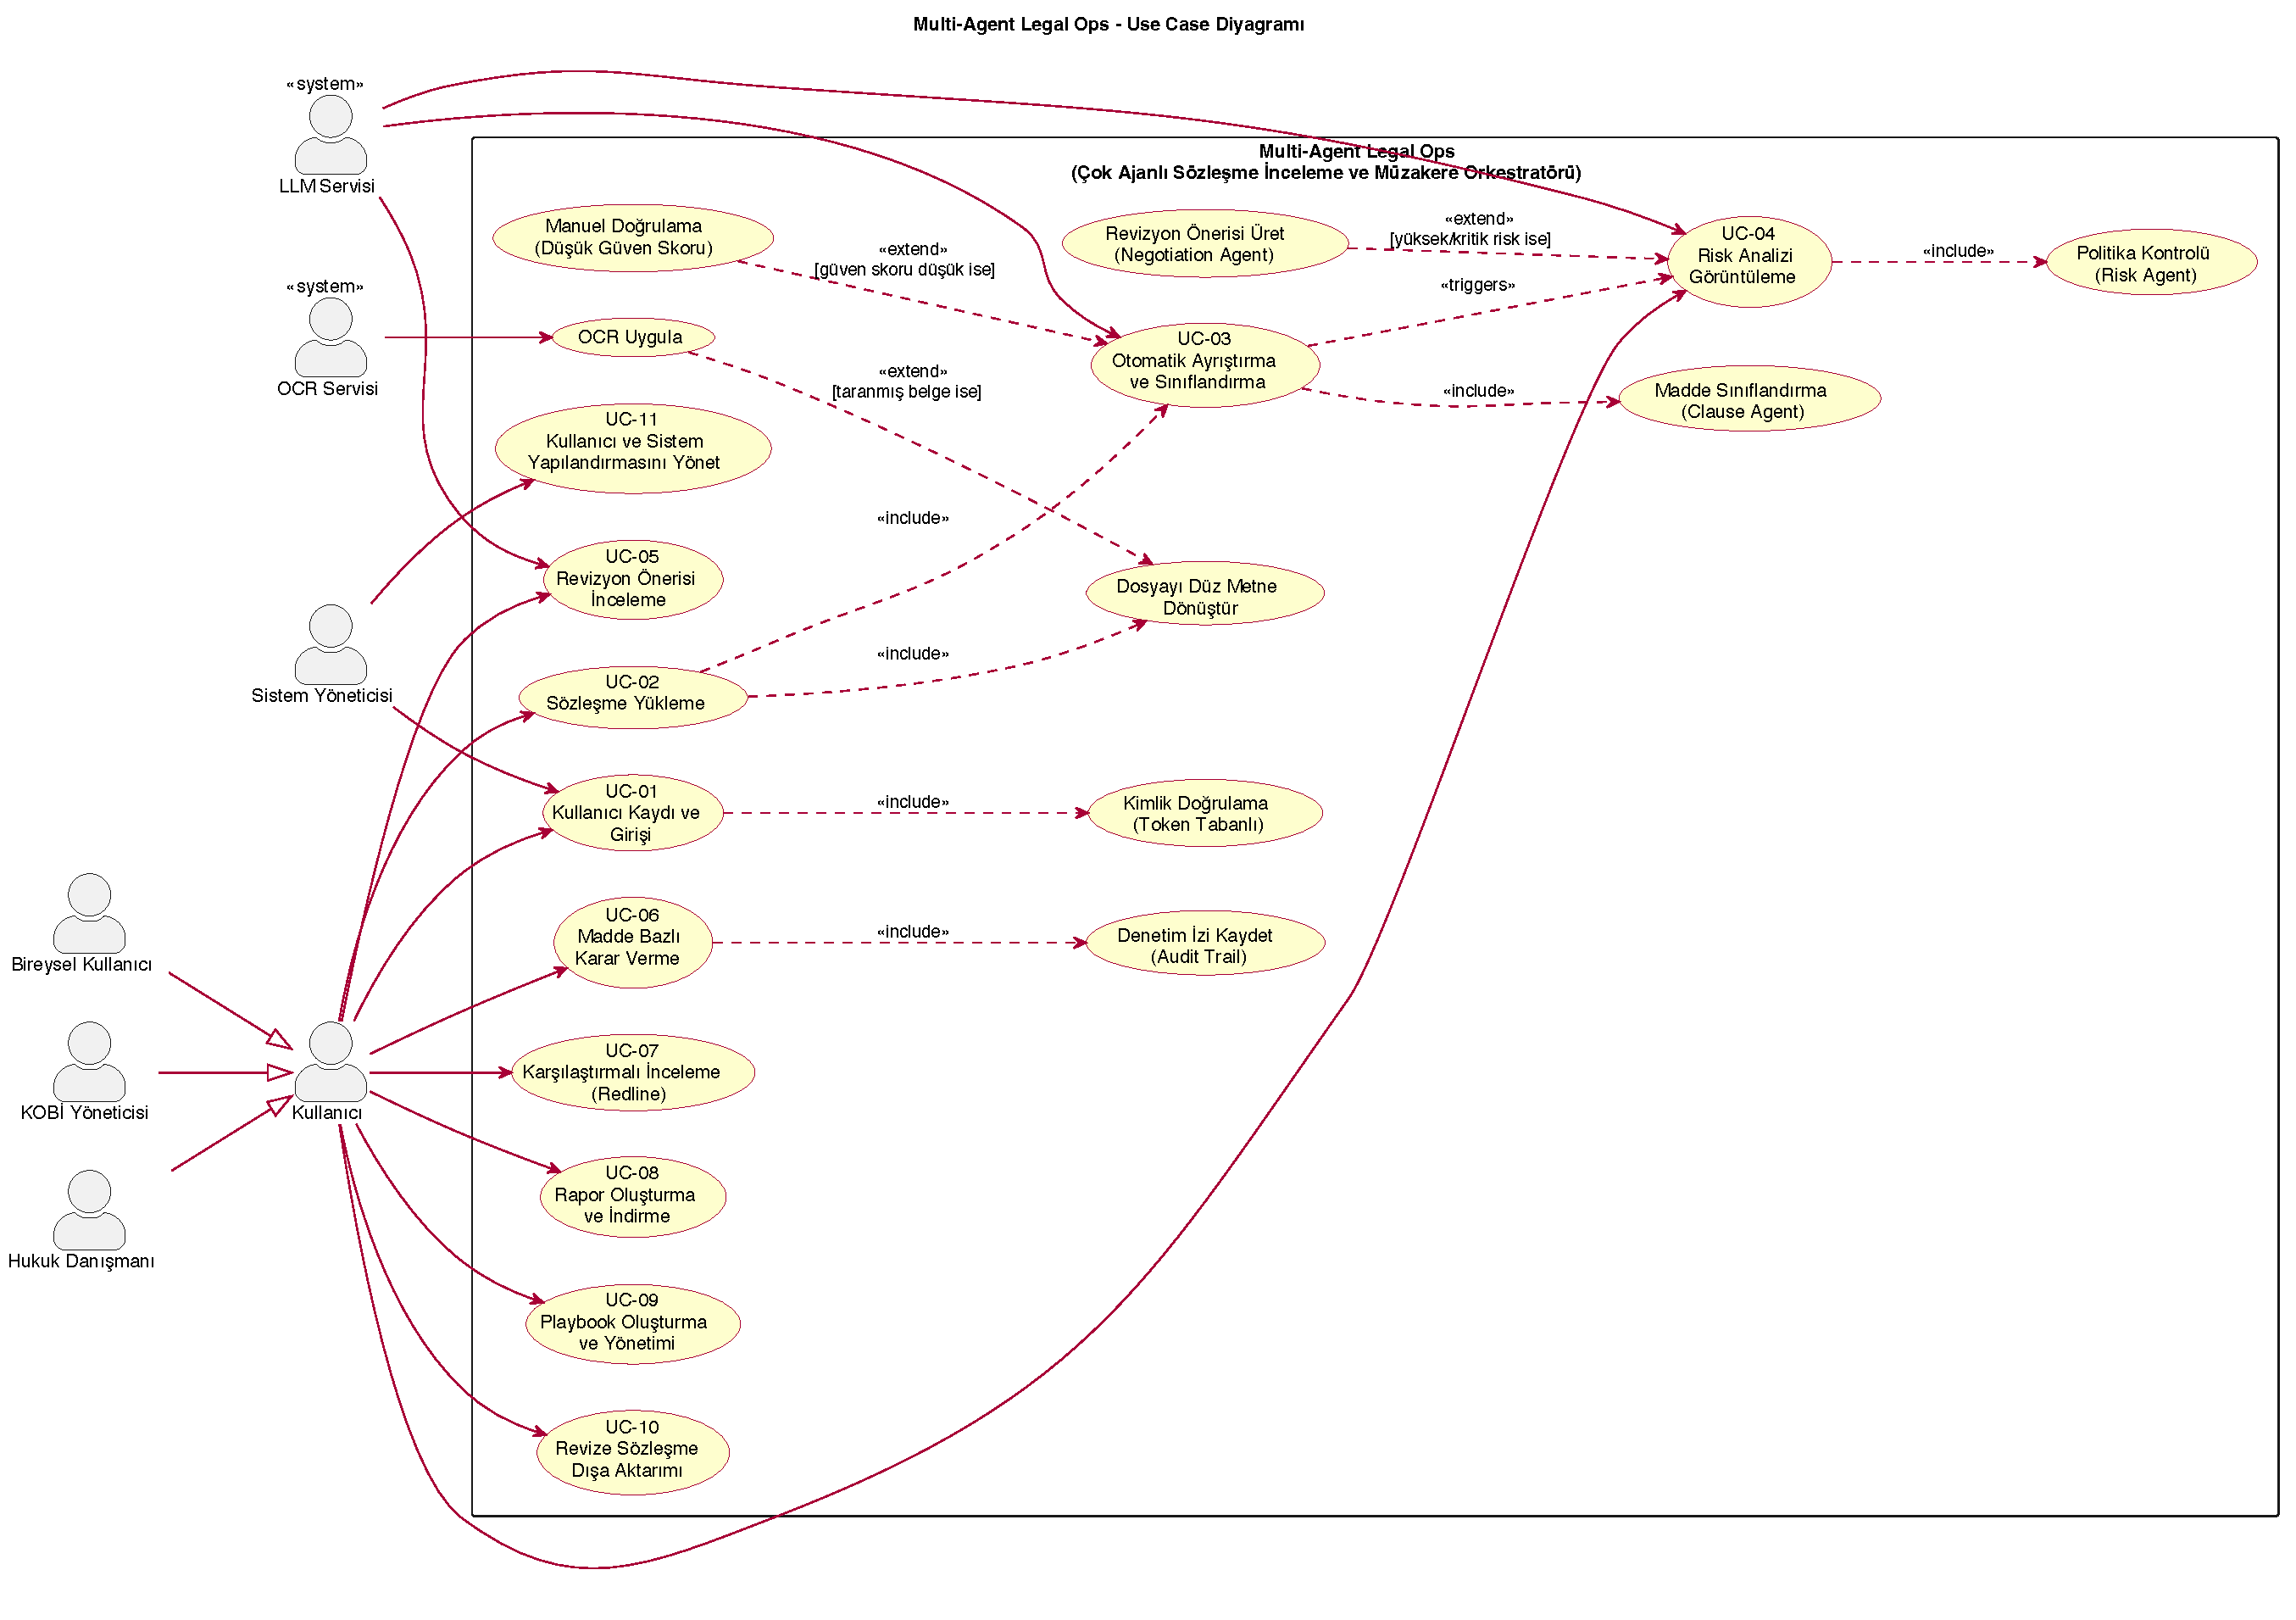
\includegraphics{Lagent Use Case Diyagramı.pdf}}
    \caption{Genel Kullanım Senaryosu (Use Case) Diyagramı}
    \label{fig:use-case-genel}
\end{figure}
\subsubsection{Kullanım Senaryoları Tablosu}

\begin{longtable}{|c|p{4cm}|p{8.5cm}|}
\hline
\textbf{ID} & \textbf{Senaryo} & \textbf{Açıklama} \\
\hline
\endfirsthead
\hline
\textbf{ID} & \textbf{Senaryo} & \textbf{Açıklama} \\
\hline
\endhead
UC-01 & Kullanıcı Kaydı ve Girişi & Kullanıcı sisteme kayıt olur ve kimlik doğrulaması ile giriş yapar. \\
\hline
UC-02 & Sözleşme Yükleme & Kullanıcı, incelenmesini istediği sözleşme dosyasını sisteme yükler. \\
\hline
UC-03 & Otomatik Ayrıştırma ve Sınıflandırma & Sistem, yüklenen sözleşmeyi maddelere ayırır ve her maddeyi hukuki kategorilere sınıflandırır. \\
\hline
UC-04 & Risk Analizi Görüntüleme & Kullanıcı, her maddenin risk seviyesini, risk gerekçesini ve politika uyumluluk durumunu inceler. \\
\hline
UC-05 & Revizyon Önerisi İnceleme & Kullanıcı, riskli maddeler için üretilen alternatif ifadeleri görüntüler, karşılaştırır ve değerlendirir. \\
\hline
UC-06 & Madde Bazlı Karar Verme & Kullanıcı, her madde için onay, red veya yeniden revize kararı verir ve gerekirse yorum ekler. \\
\hline
UC-07 & Karşılaştırmalı İnceleme (Redline) & Kullanıcı, orijinal ve önerilen metinleri yan yana karşılaştırmalı görünümde inceler. \\
\hline
UC-08 & Rapor Oluşturma ve İndirme & Kullanıcı, inceleme sonuçlarını özet veya detaylı rapor olarak görüntüler ve dosya formatında indirir. \\
\hline
UC-09 & Playbook Oluşturma ve Yönetimi & Kullanıcı, kendi sözleşme politikalarını tanımlar, düzenler ve analiz için etkinleştirir. \\
\hline
UC-10 & Revize Sözleşme Dışa Aktarımı & Kullanıcı, onaylanan değişikliklerle güncellenmiş sözleşme taslağını dosya olarak indirir. \\
\hline
UC-11 & Kullanıcı ve Sistem Yapılandırması Yönetimi & Sistem yöneticisi, kullanıcı hesaplarını ve sistem yapılandırma parametrelerini yönetir. \\
\hline
\end{longtable}

\subsubsection{Kullanım Senaryosu Diyagramları}
Aşağıda her bir kullanım senaryosunun detaylı diyagramları yer almaktadır.
\begin{landscape}
\centering

% Her bir görsel için bu bloğu kullanabilirsin:
\begin{minipage}{\linewidth}
    \centering
    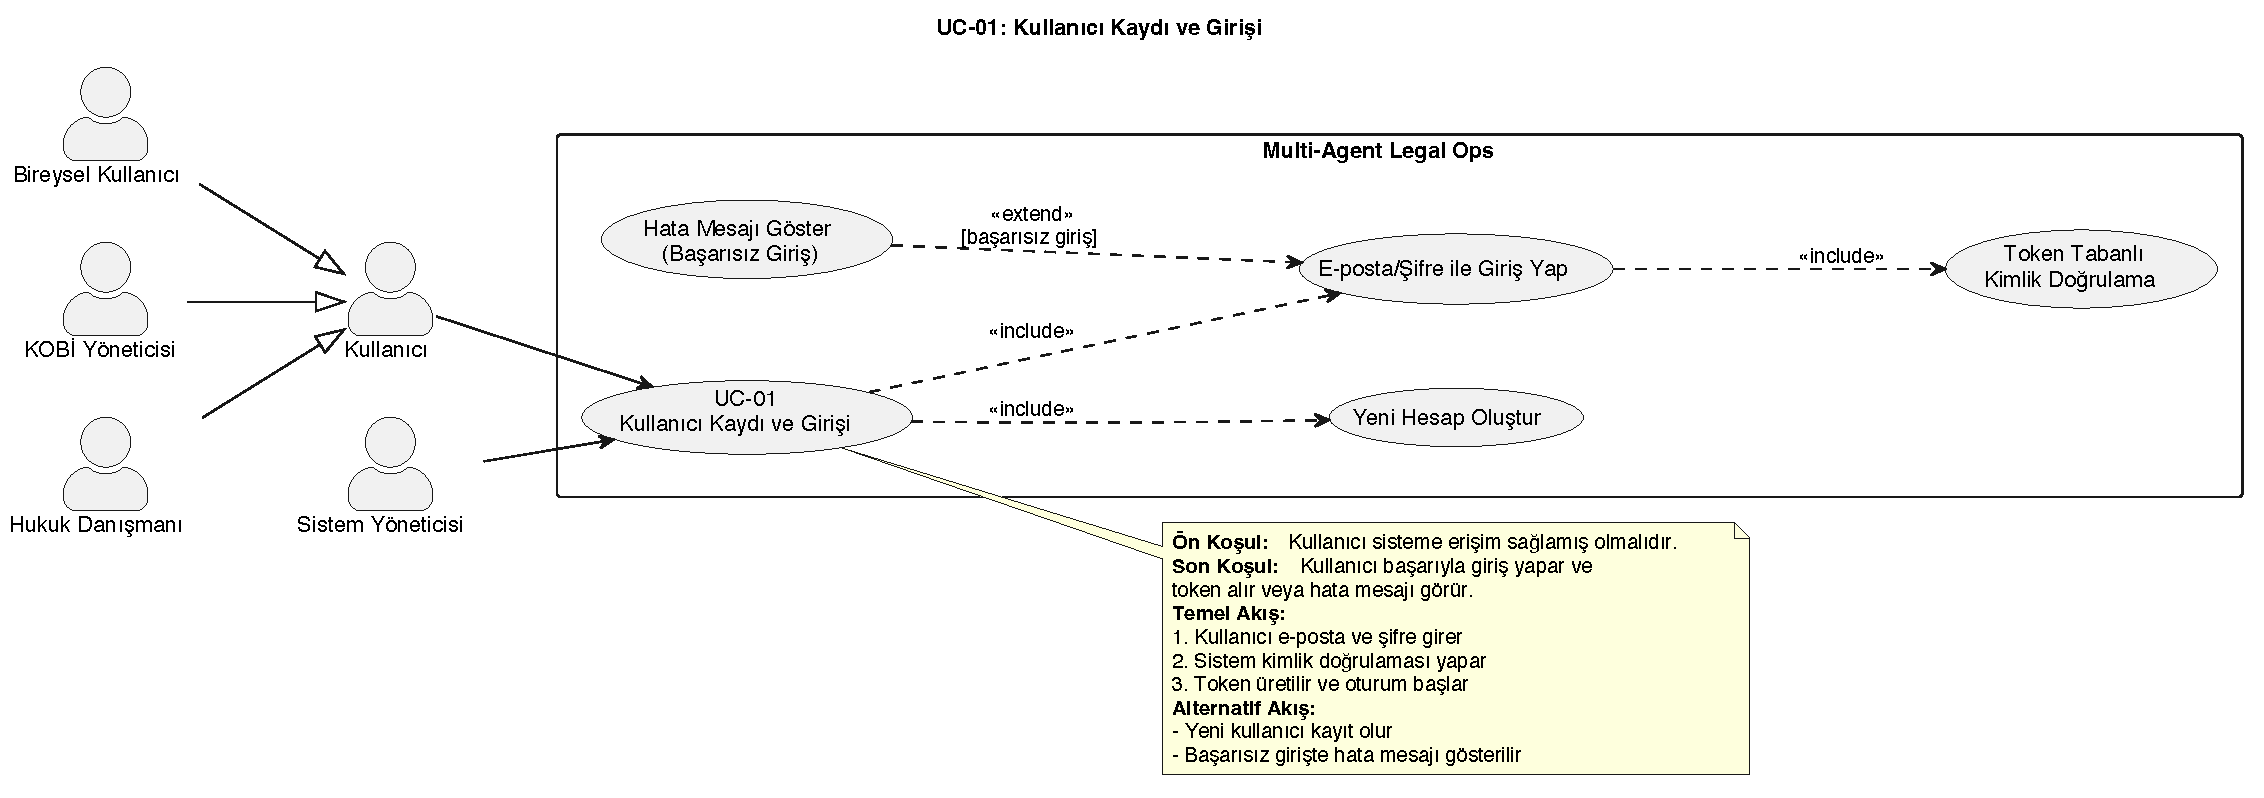
\includegraphics[height=0.85\textheight, width=0.95\linewidth, keepaspectratio]{UC-01.pdf}
    \captionof{figure}{UC-01: Kullanıcı Kaydı ve Girişi}
    \label{fig:uc01}
\end{minipage}
\clearpage

\begin{minipage}{\linewidth}
    \centering
    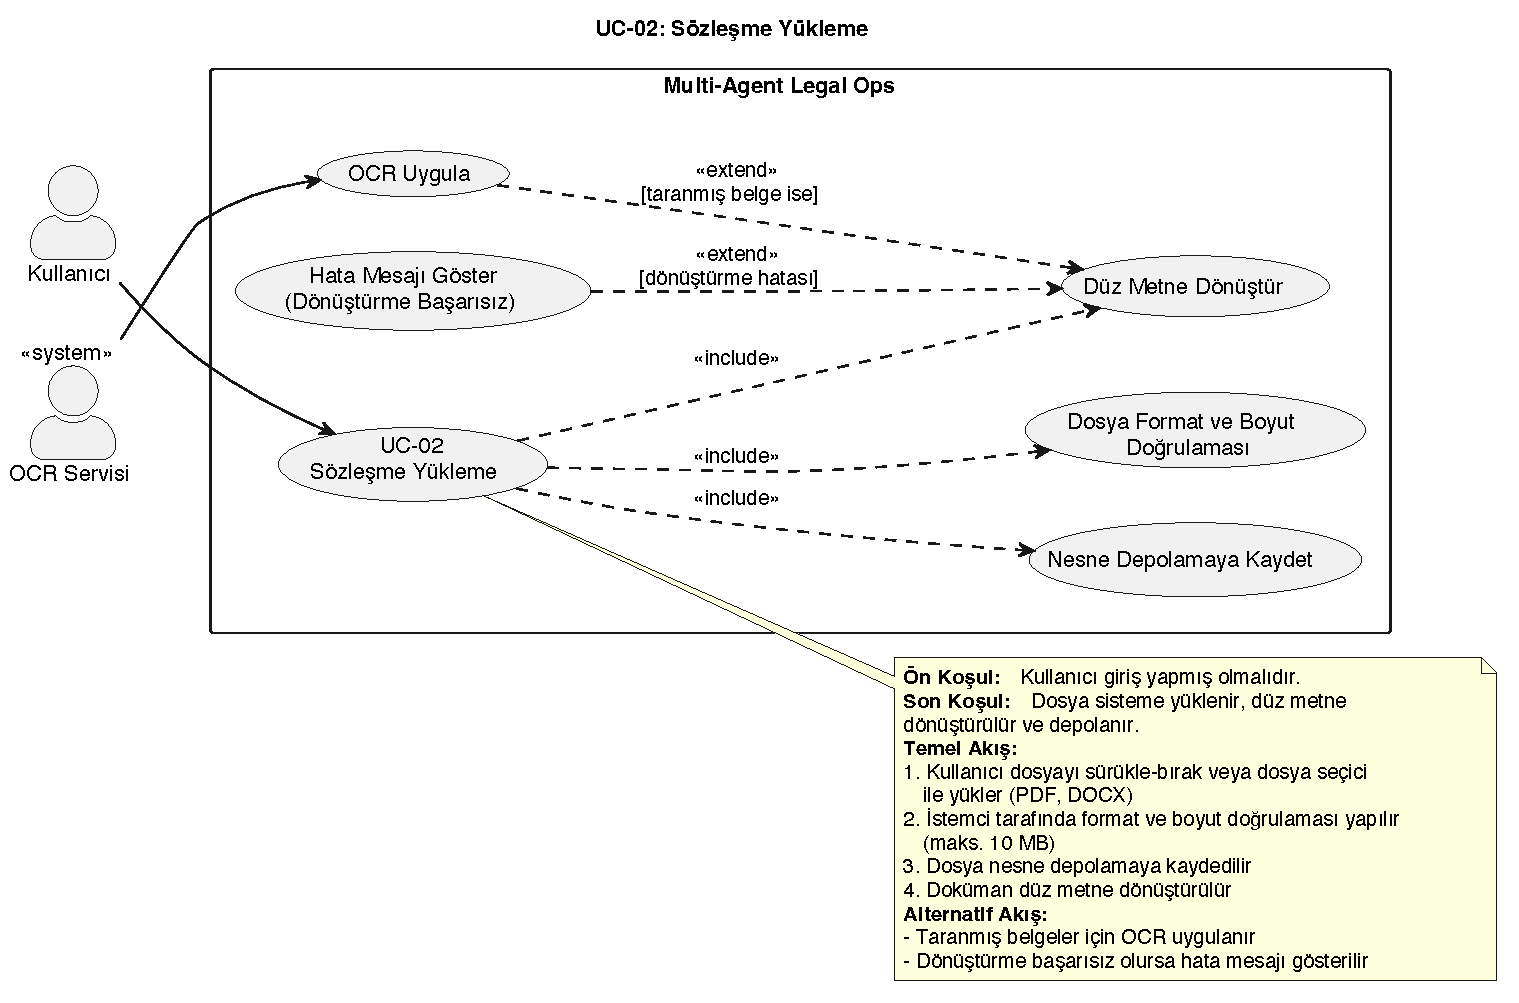
\includegraphics[height=0.85\textheight, width=0.95\linewidth, keepaspectratio]{UC-02.pdf}
    \captionof{figure}{UC-02: Sözleşme Yükleme}
    \label{fig:uc02}
\end{minipage}
\clearpage

\begin{minipage}{\linewidth}
    \centering
    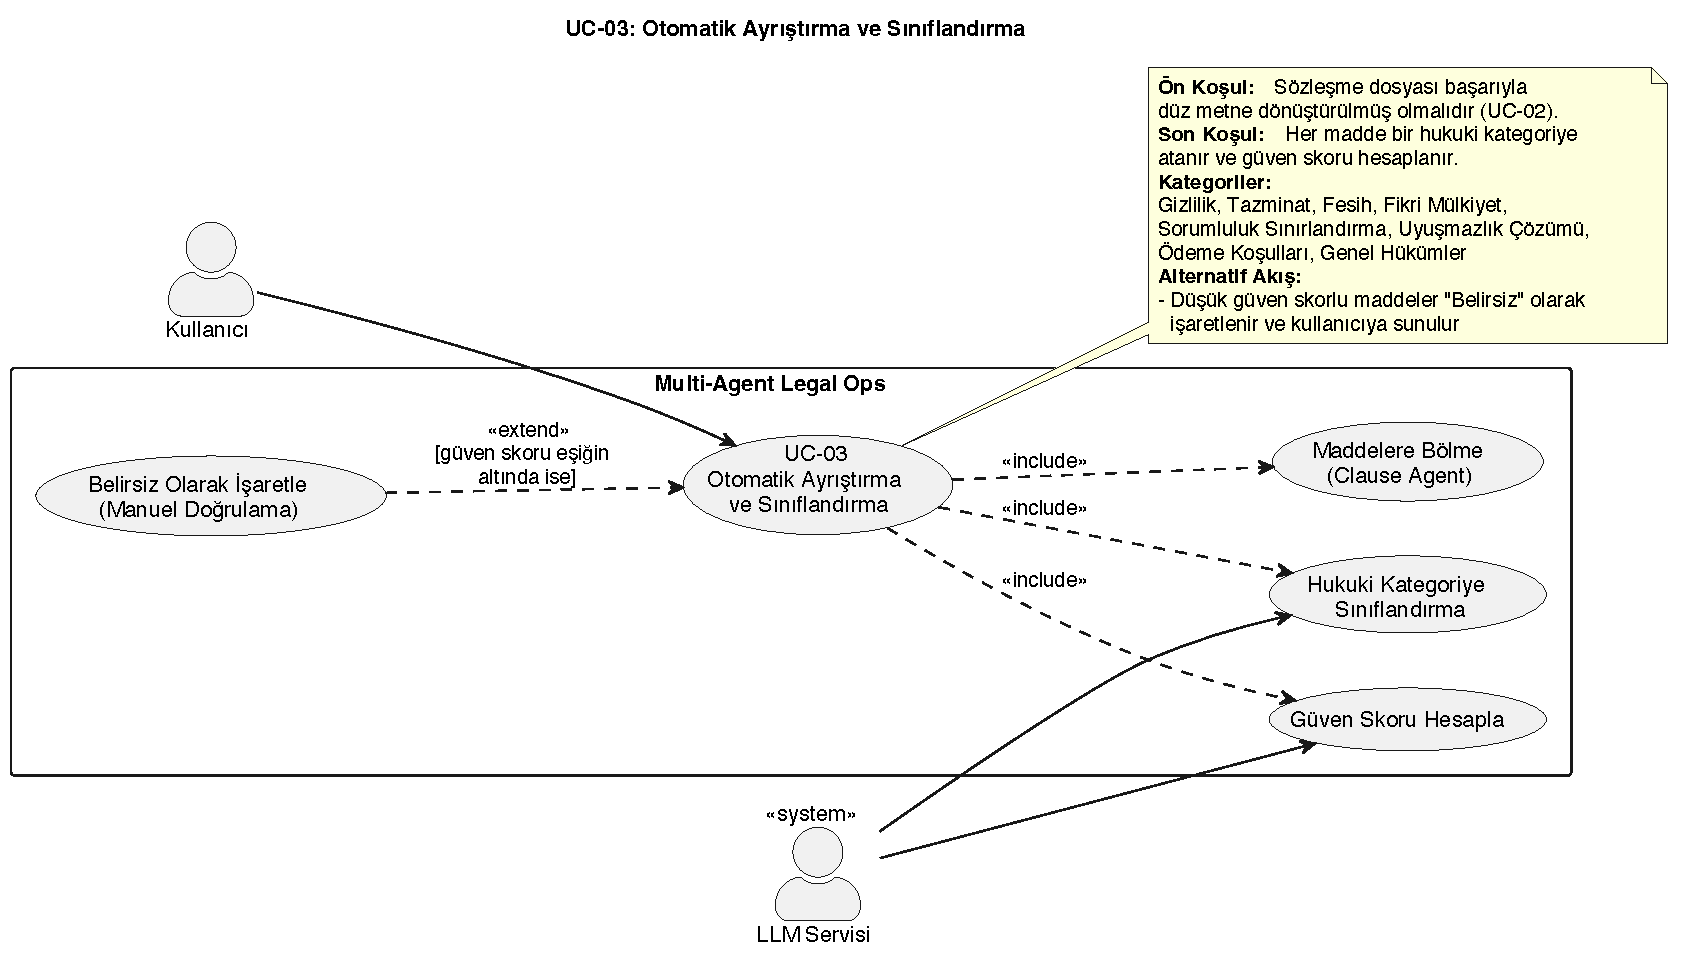
\includegraphics[height=0.85\textheight, width=0.95\linewidth, keepaspectratio]{UC-03.pdf}
    \captionof{figure}{UC-03: Otomatik Ayrıştırma ve Sınıflandırma}
    \label{fig:uc03}
\end{minipage}
\clearpage

\begin{minipage}{\linewidth}
    \centering
    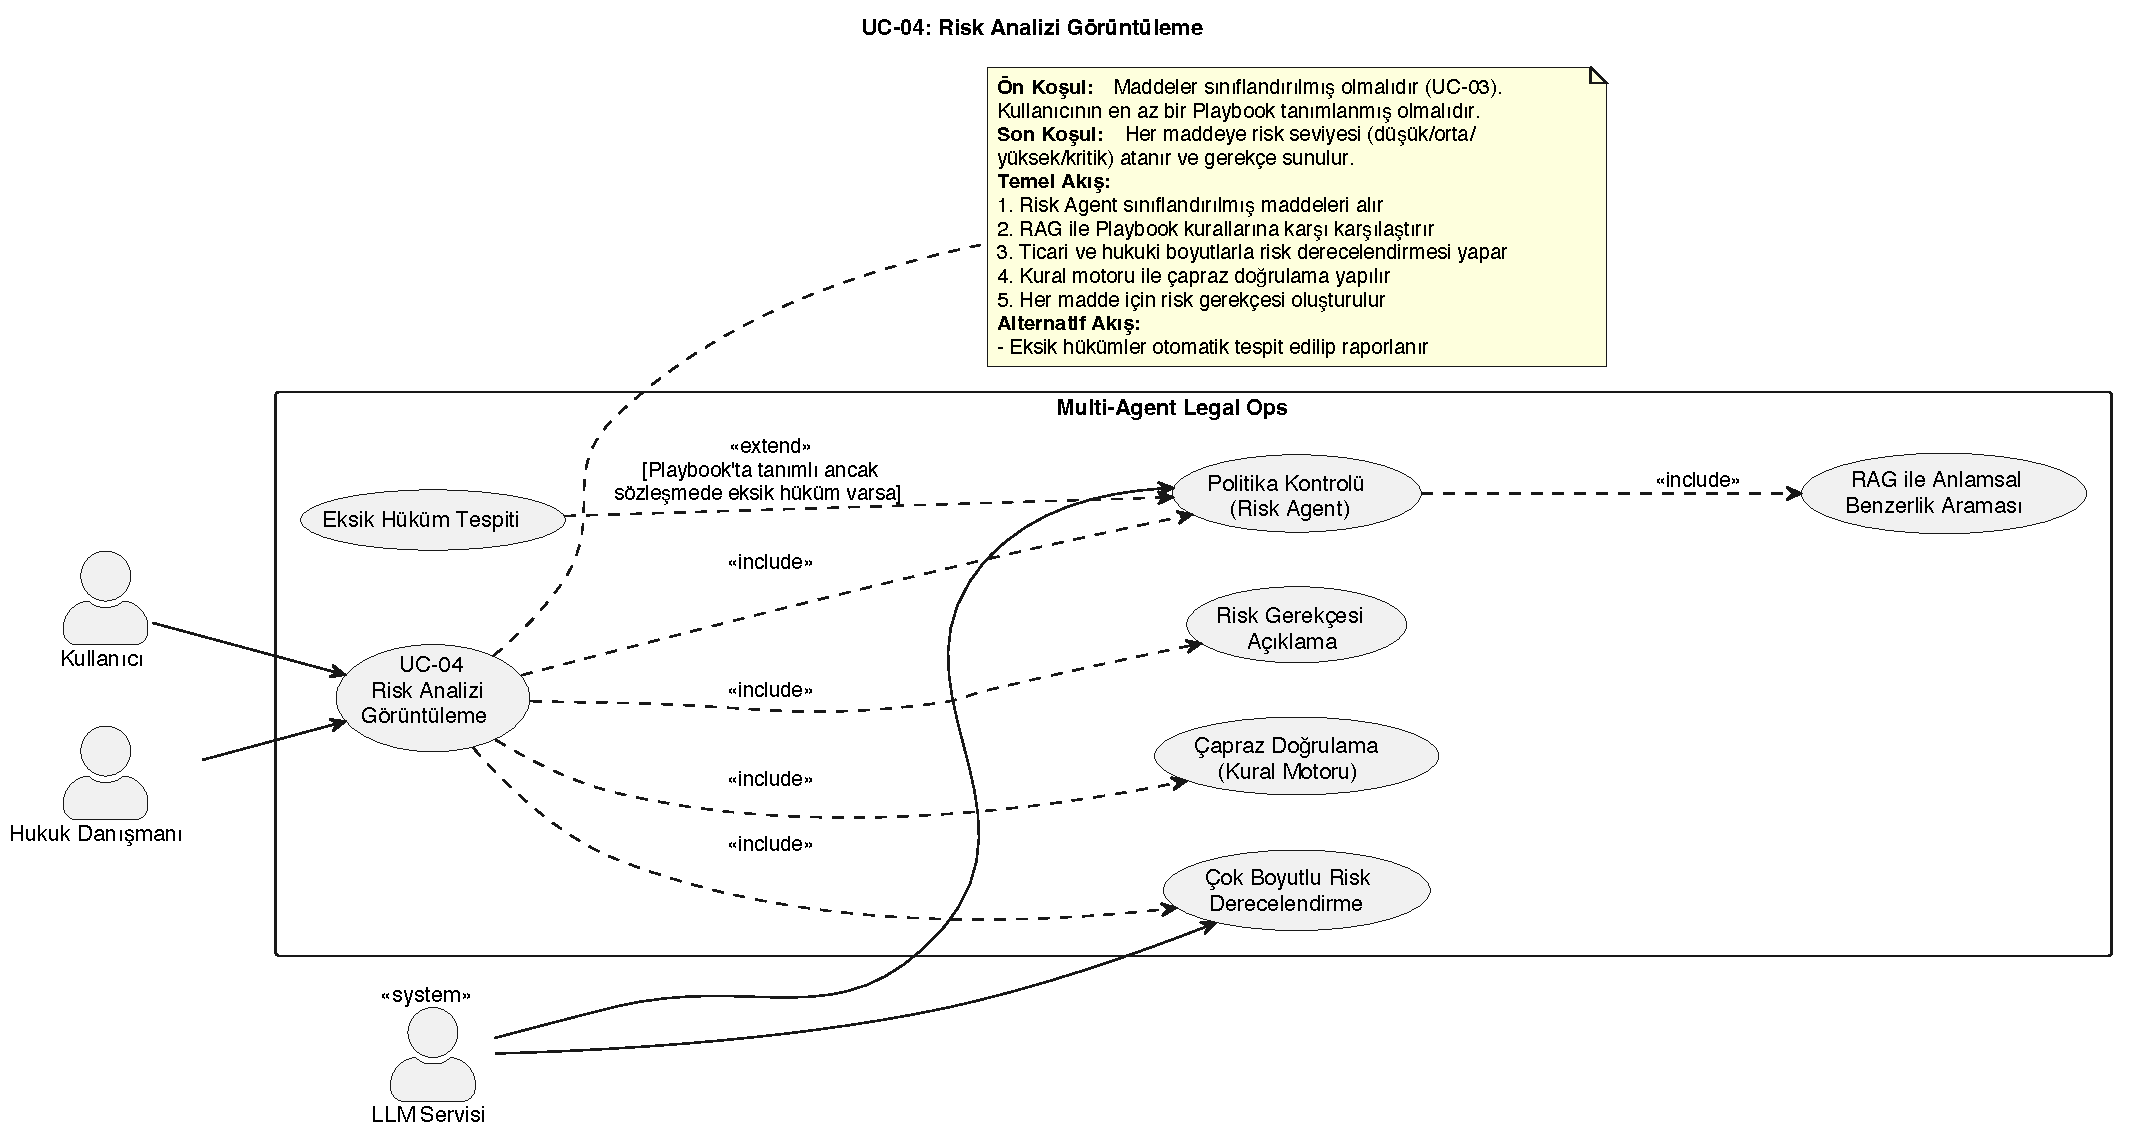
\includegraphics[height=0.85\textheight, width=0.95\linewidth, keepaspectratio]{UC-04.pdf}
    \captionof{figure}{UC-04: Risk Analizi Görüntüleme}
    \label{fig:uc04}
\end{minipage}
\clearpage

\begin{minipage}{\linewidth}
    \centering
    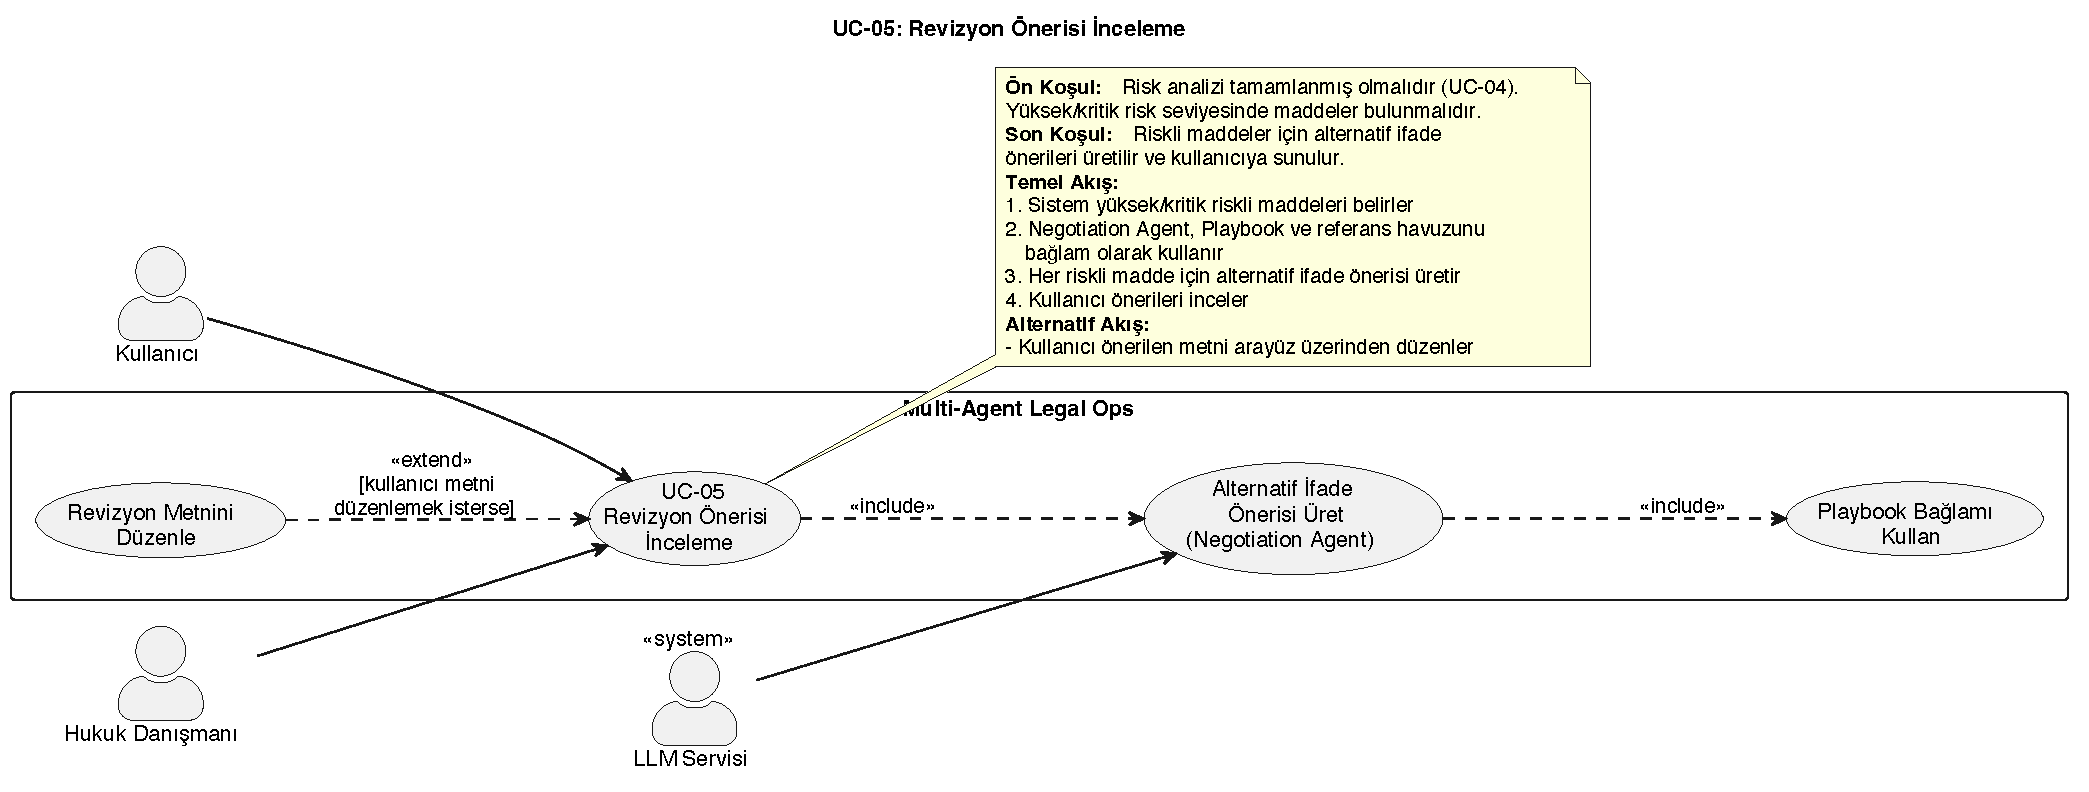
\includegraphics[height=0.85\textheight, width=0.95\linewidth, keepaspectratio]{UC-05.pdf}
    \captionof{figure}{UC-05: Revizyon Önerisi İnceleme}
    \label{fig:uc05}
\end{minipage}
\clearpage

\begin{minipage}{\linewidth}
    \centering
    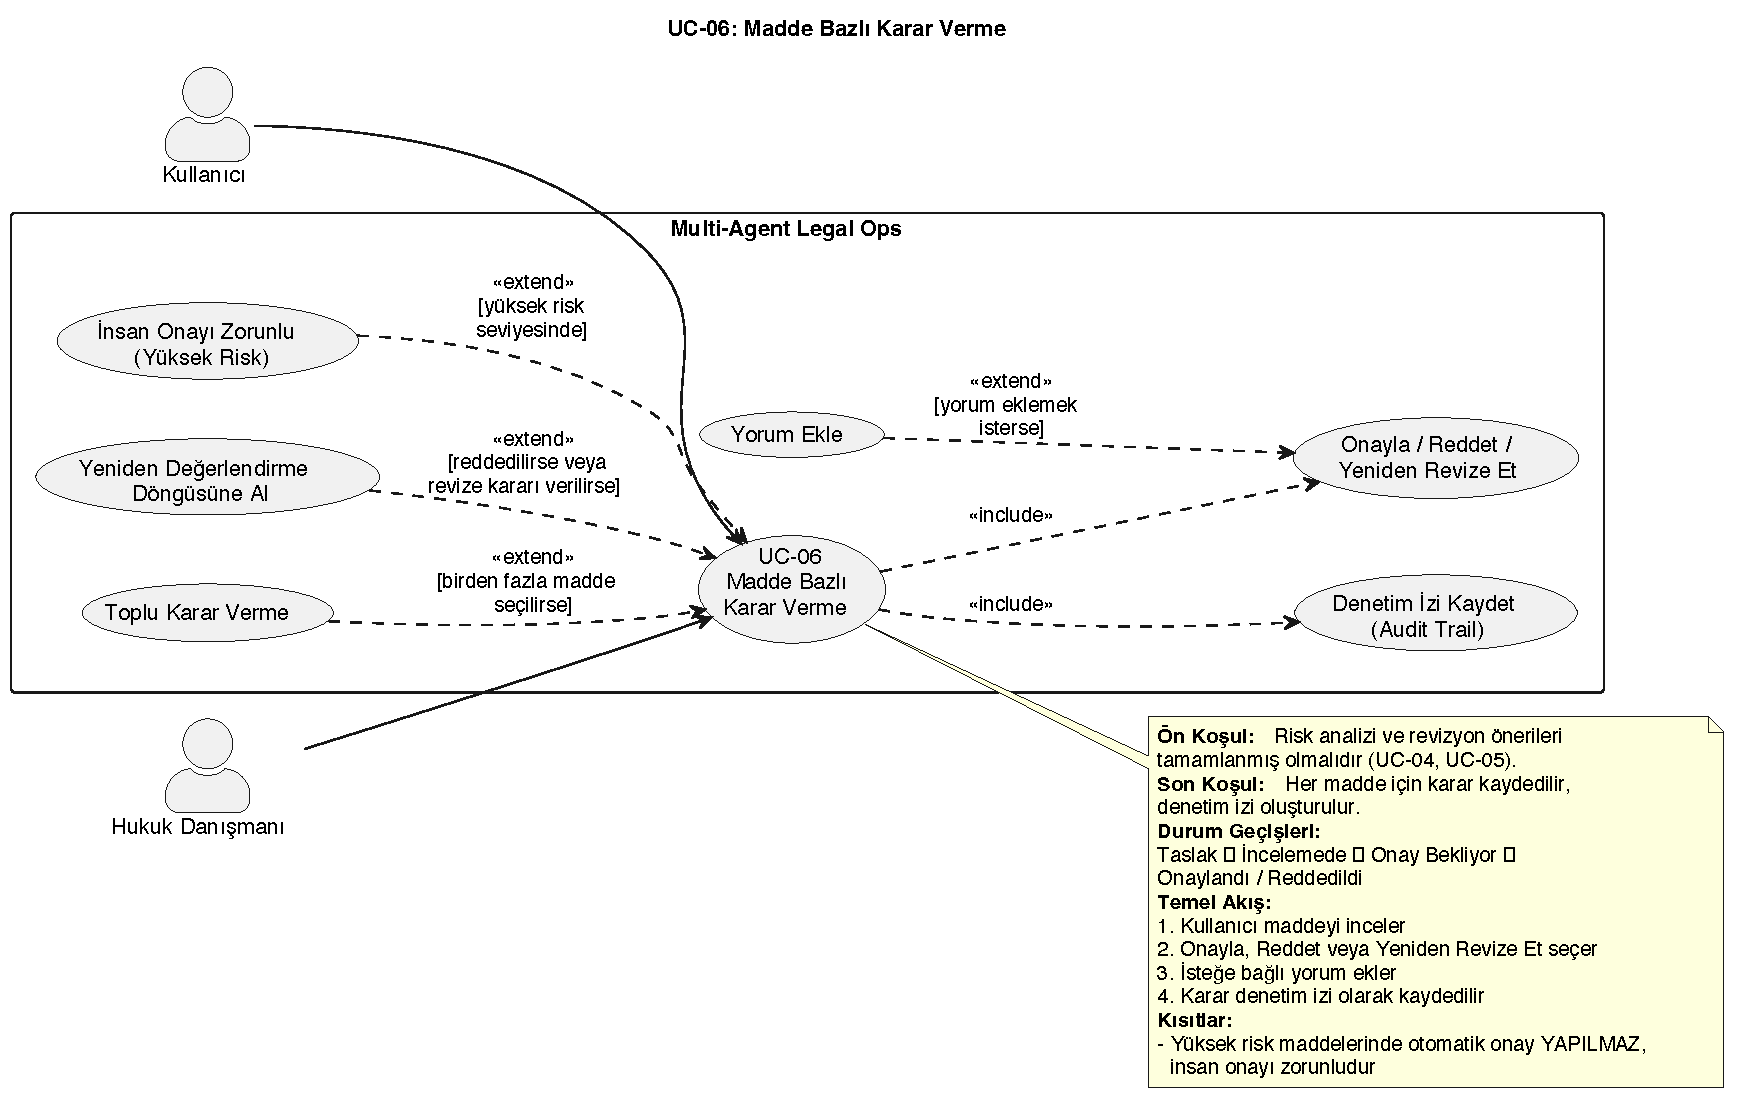
\includegraphics[height=0.85\textheight, width=0.95\linewidth, keepaspectratio]{UC-06.pdf}
    \captionof{figure}{UC-06: Madde Bazlı Karar Verme}
    \label{fig:uc06}
\end{minipage}
\clearpage

\begin{minipage}{\linewidth}
    \centering
    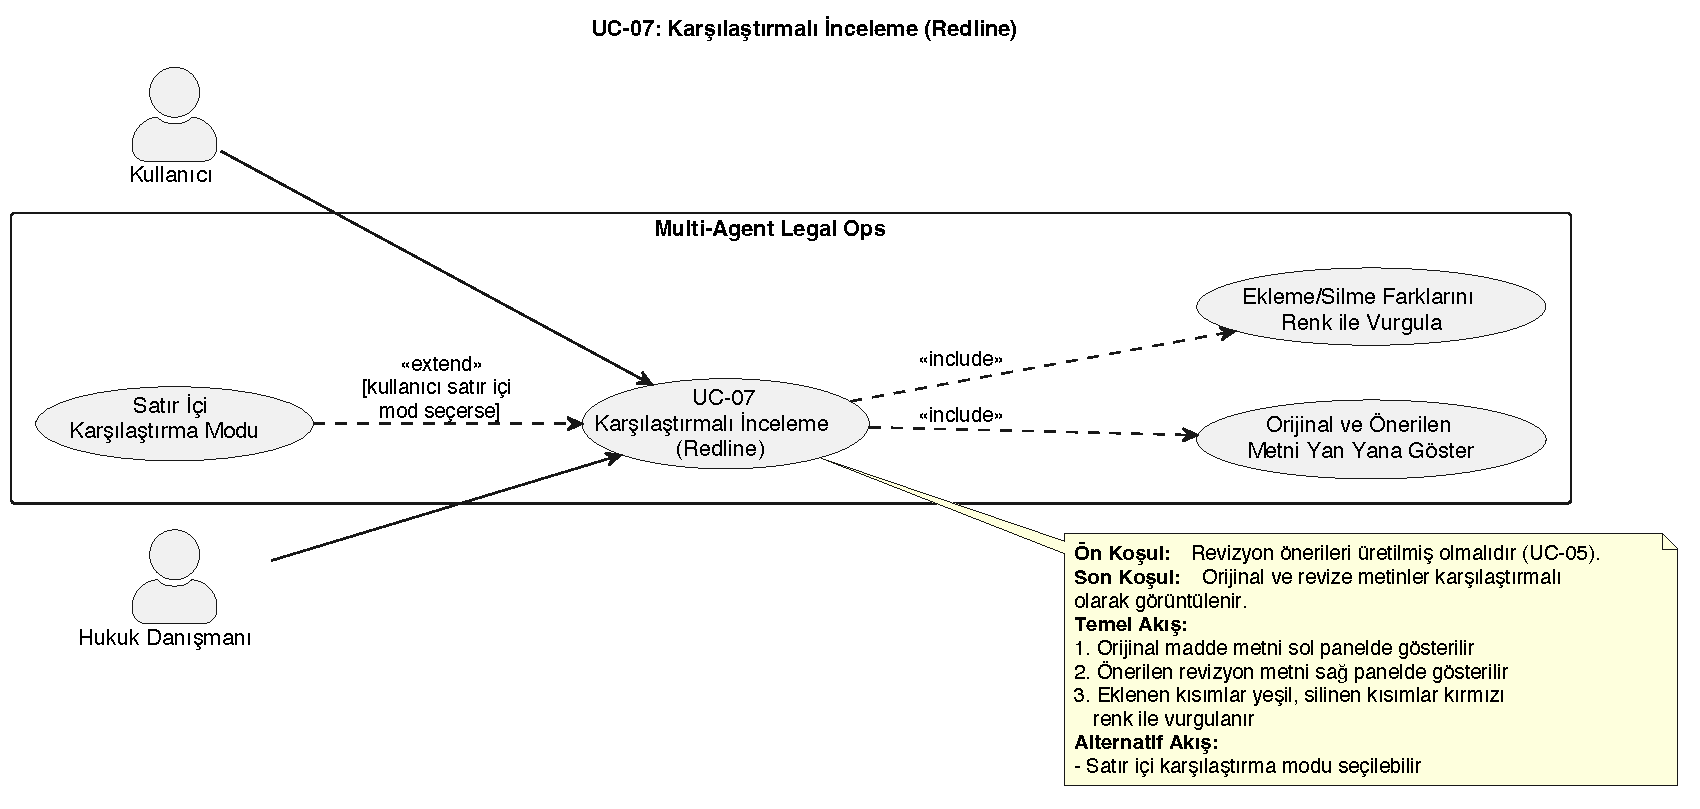
\includegraphics[height=0.85\textheight, width=0.95\linewidth, keepaspectratio]{UC-07.pdf}
    \captionof{figure}{UC-07: Karşılaştırmalı İnceleme (Redline)}
    \label{fig:uc07}
\end{minipage}
\clearpage

\begin{minipage}{\linewidth}
    \centering
    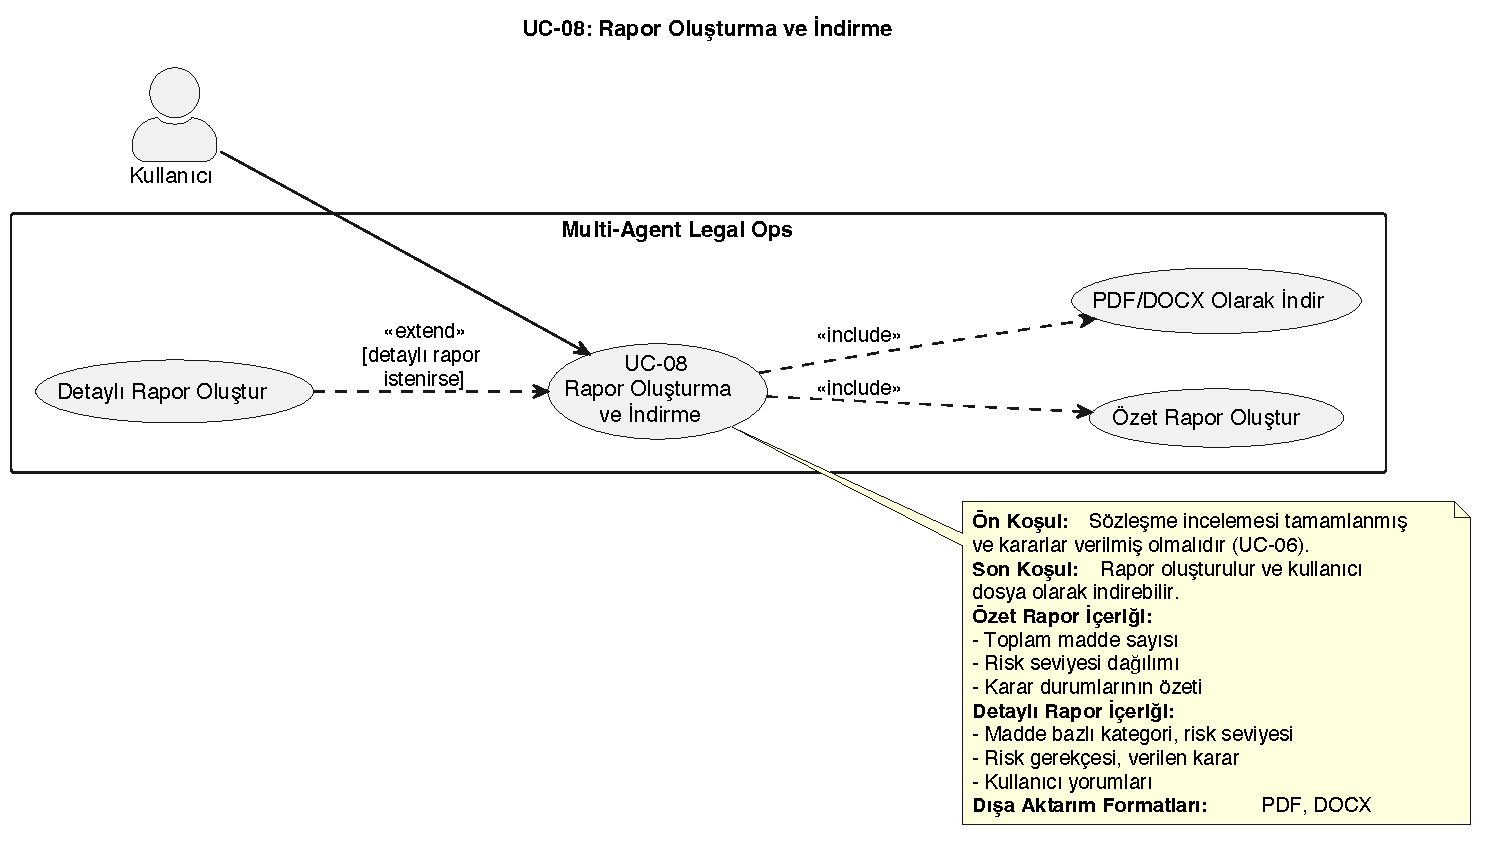
\includegraphics[height=0.85\textheight, width=0.95\linewidth, keepaspectratio]{UC-08.pdf}
    \captionof{figure}{UC-08: Rapor Oluşturma ve İndirme}
    \label{fig:uc08}
\end{minipage}
\clearpage

\begin{minipage}{\linewidth}
    \centering
    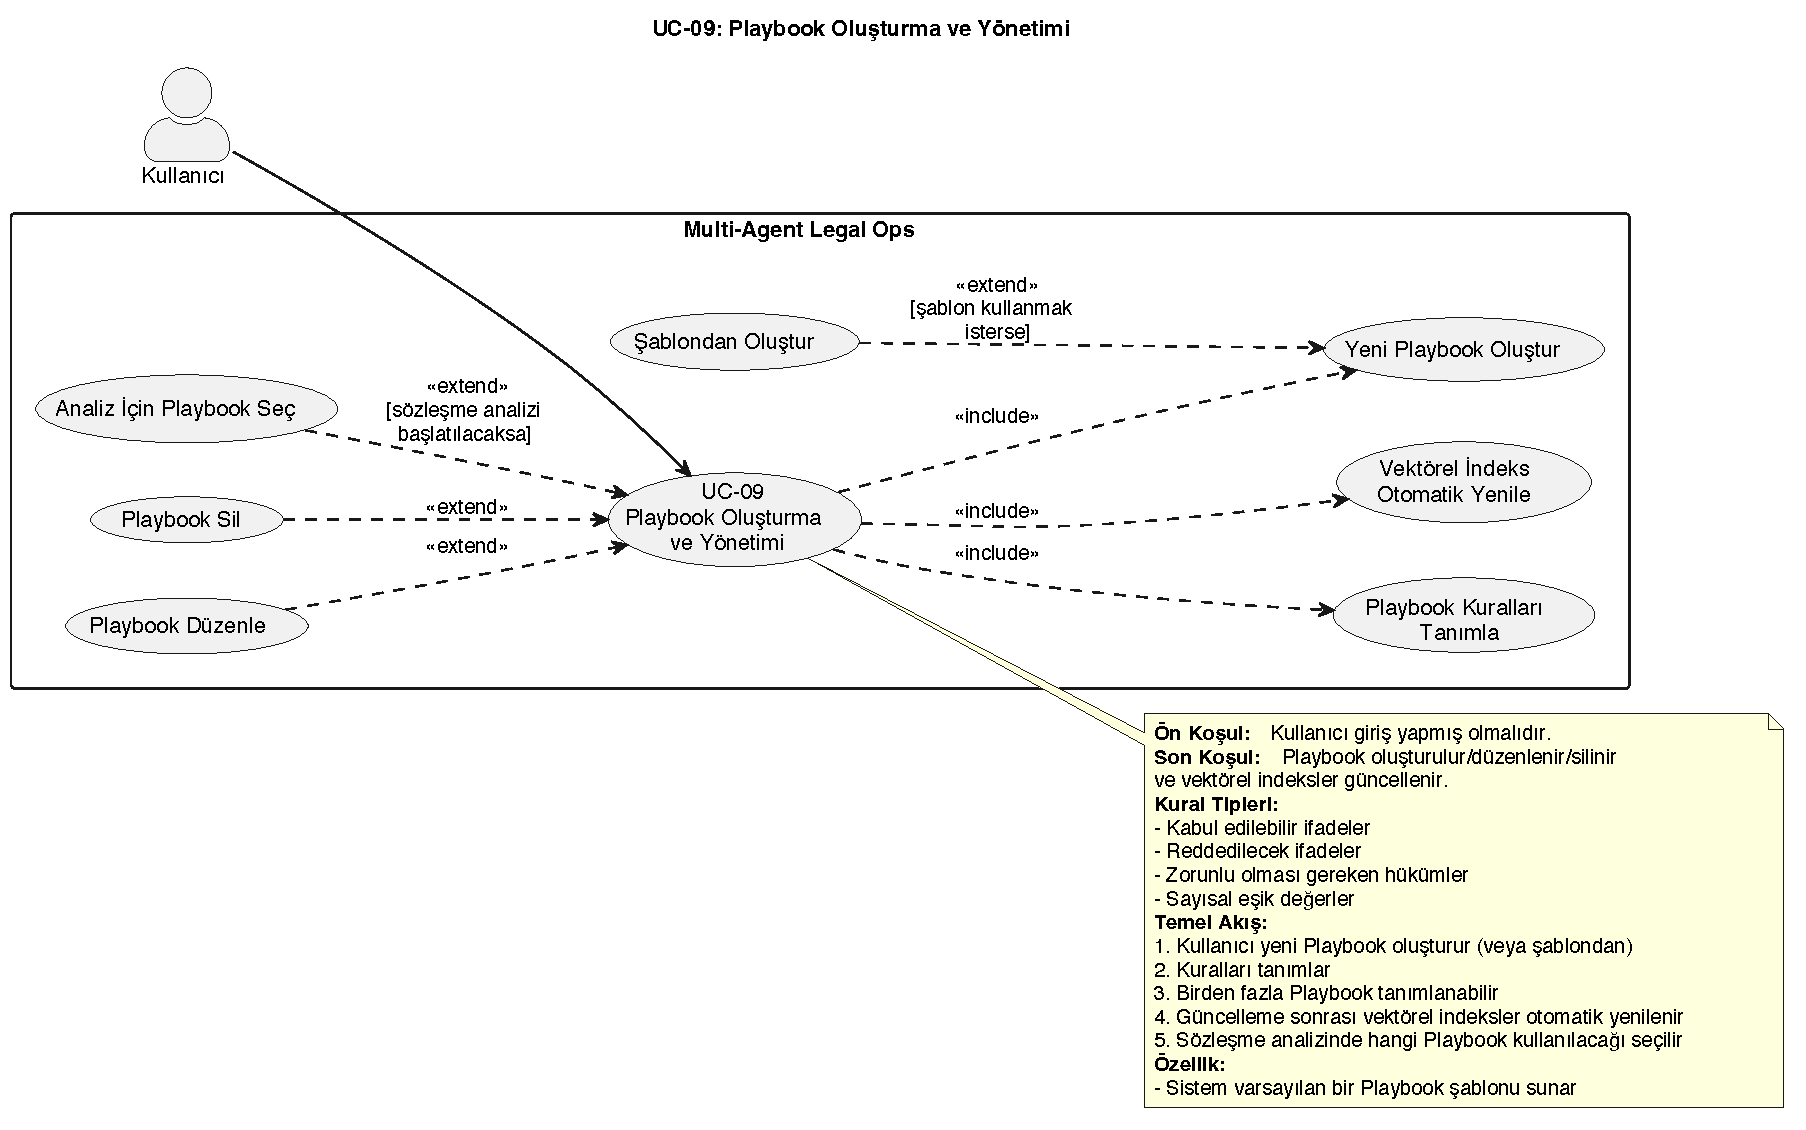
\includegraphics[height=0.85\textheight, width=0.95\linewidth, keepaspectratio]{UC-09.pdf}
    \captionof{figure}{UC-09: Playbook Oluşturma ve Yönetimi}
    \label{fig:uc09}
\end{minipage}
\clearpage

\begin{minipage}{\linewidth}
    \centering
    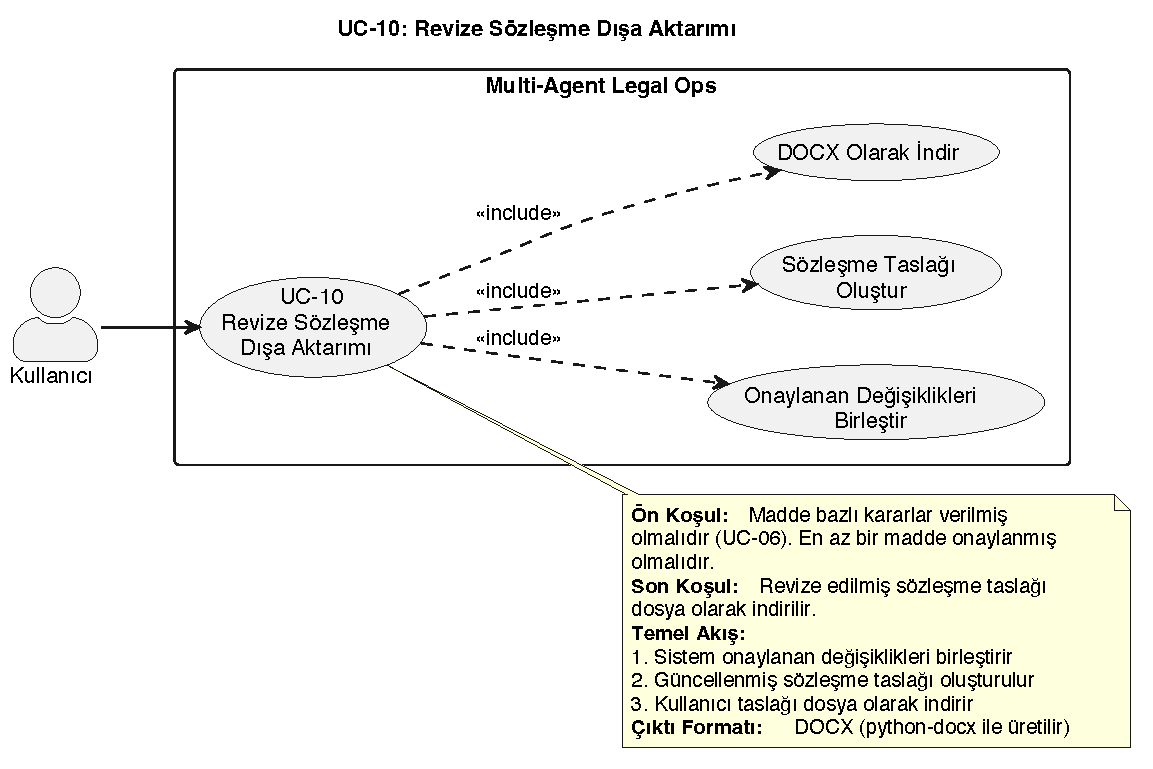
\includegraphics[height=0.85\textheight, width=0.95\linewidth, keepaspectratio]{UC-10.pdf}
    \captionof{figure}{UC-10: Revize Sözleşme Dışa Aktarımı}
    \label{fig:uc10}
\end{minipage}
\clearpage

\begin{minipage}{\linewidth}
    \centering
    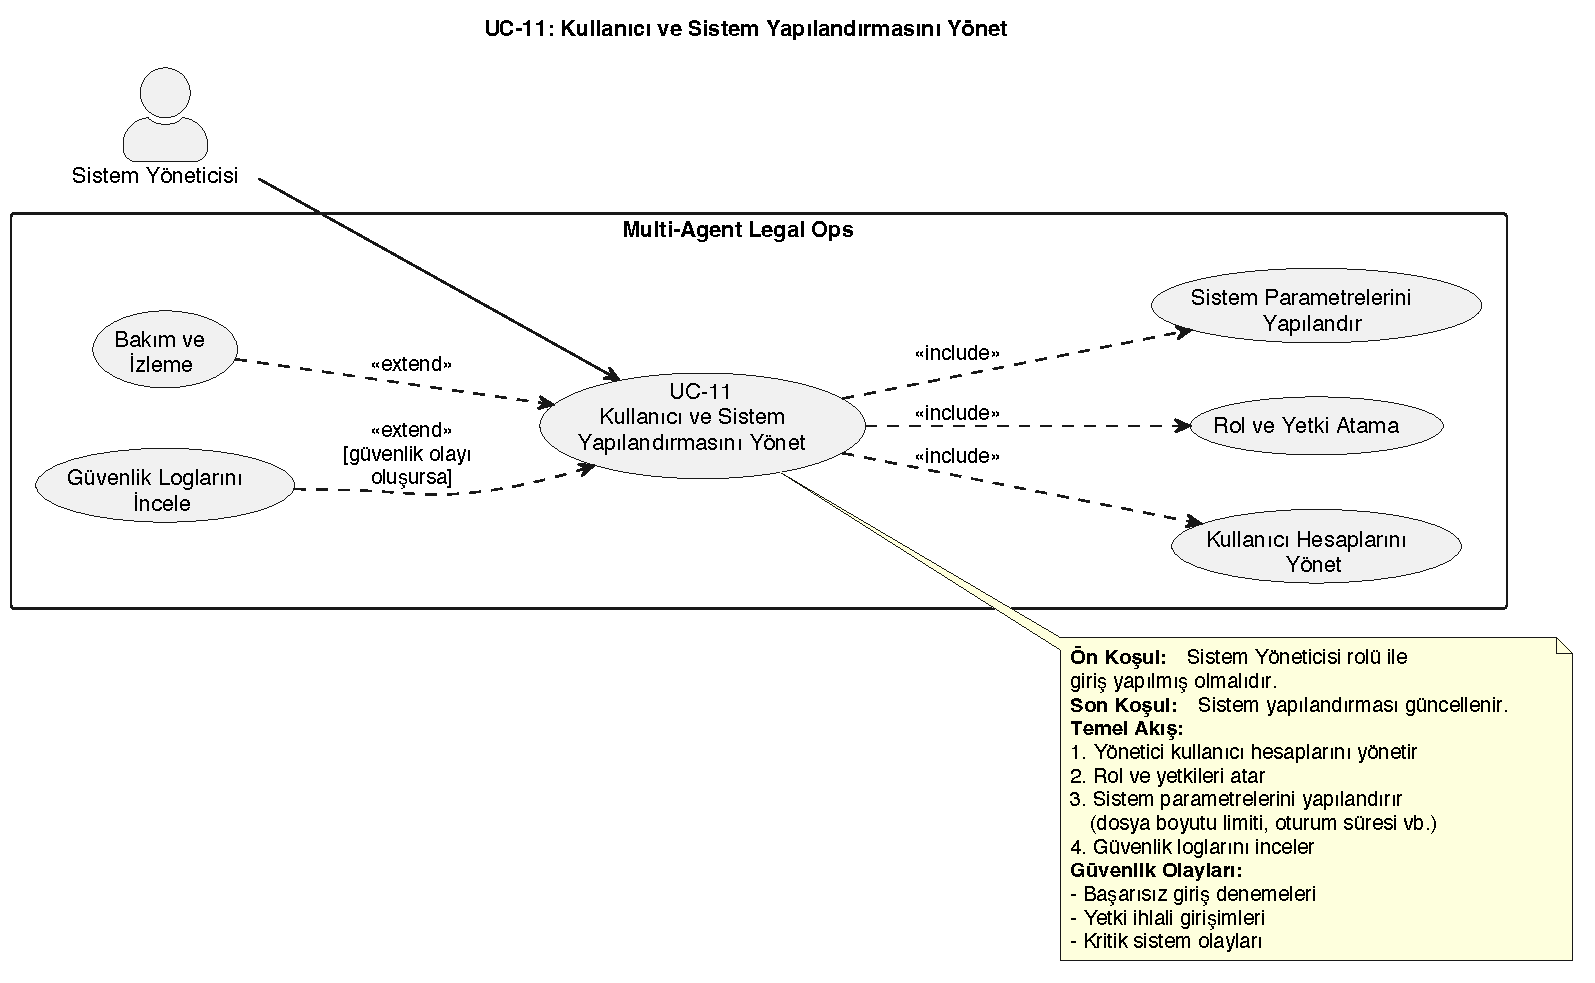
\includegraphics[height=0.85\textheight, width=0.95\linewidth, keepaspectratio]{UC-11.pdf}
    \captionof{figure}{UC-11: Kullanıcı ve Sistem Yapılandırması Yönetimi}
    \label{fig:uc11}
\end{minipage}
\clearpage

\begin{minipage}{\linewidth}
    \centering
    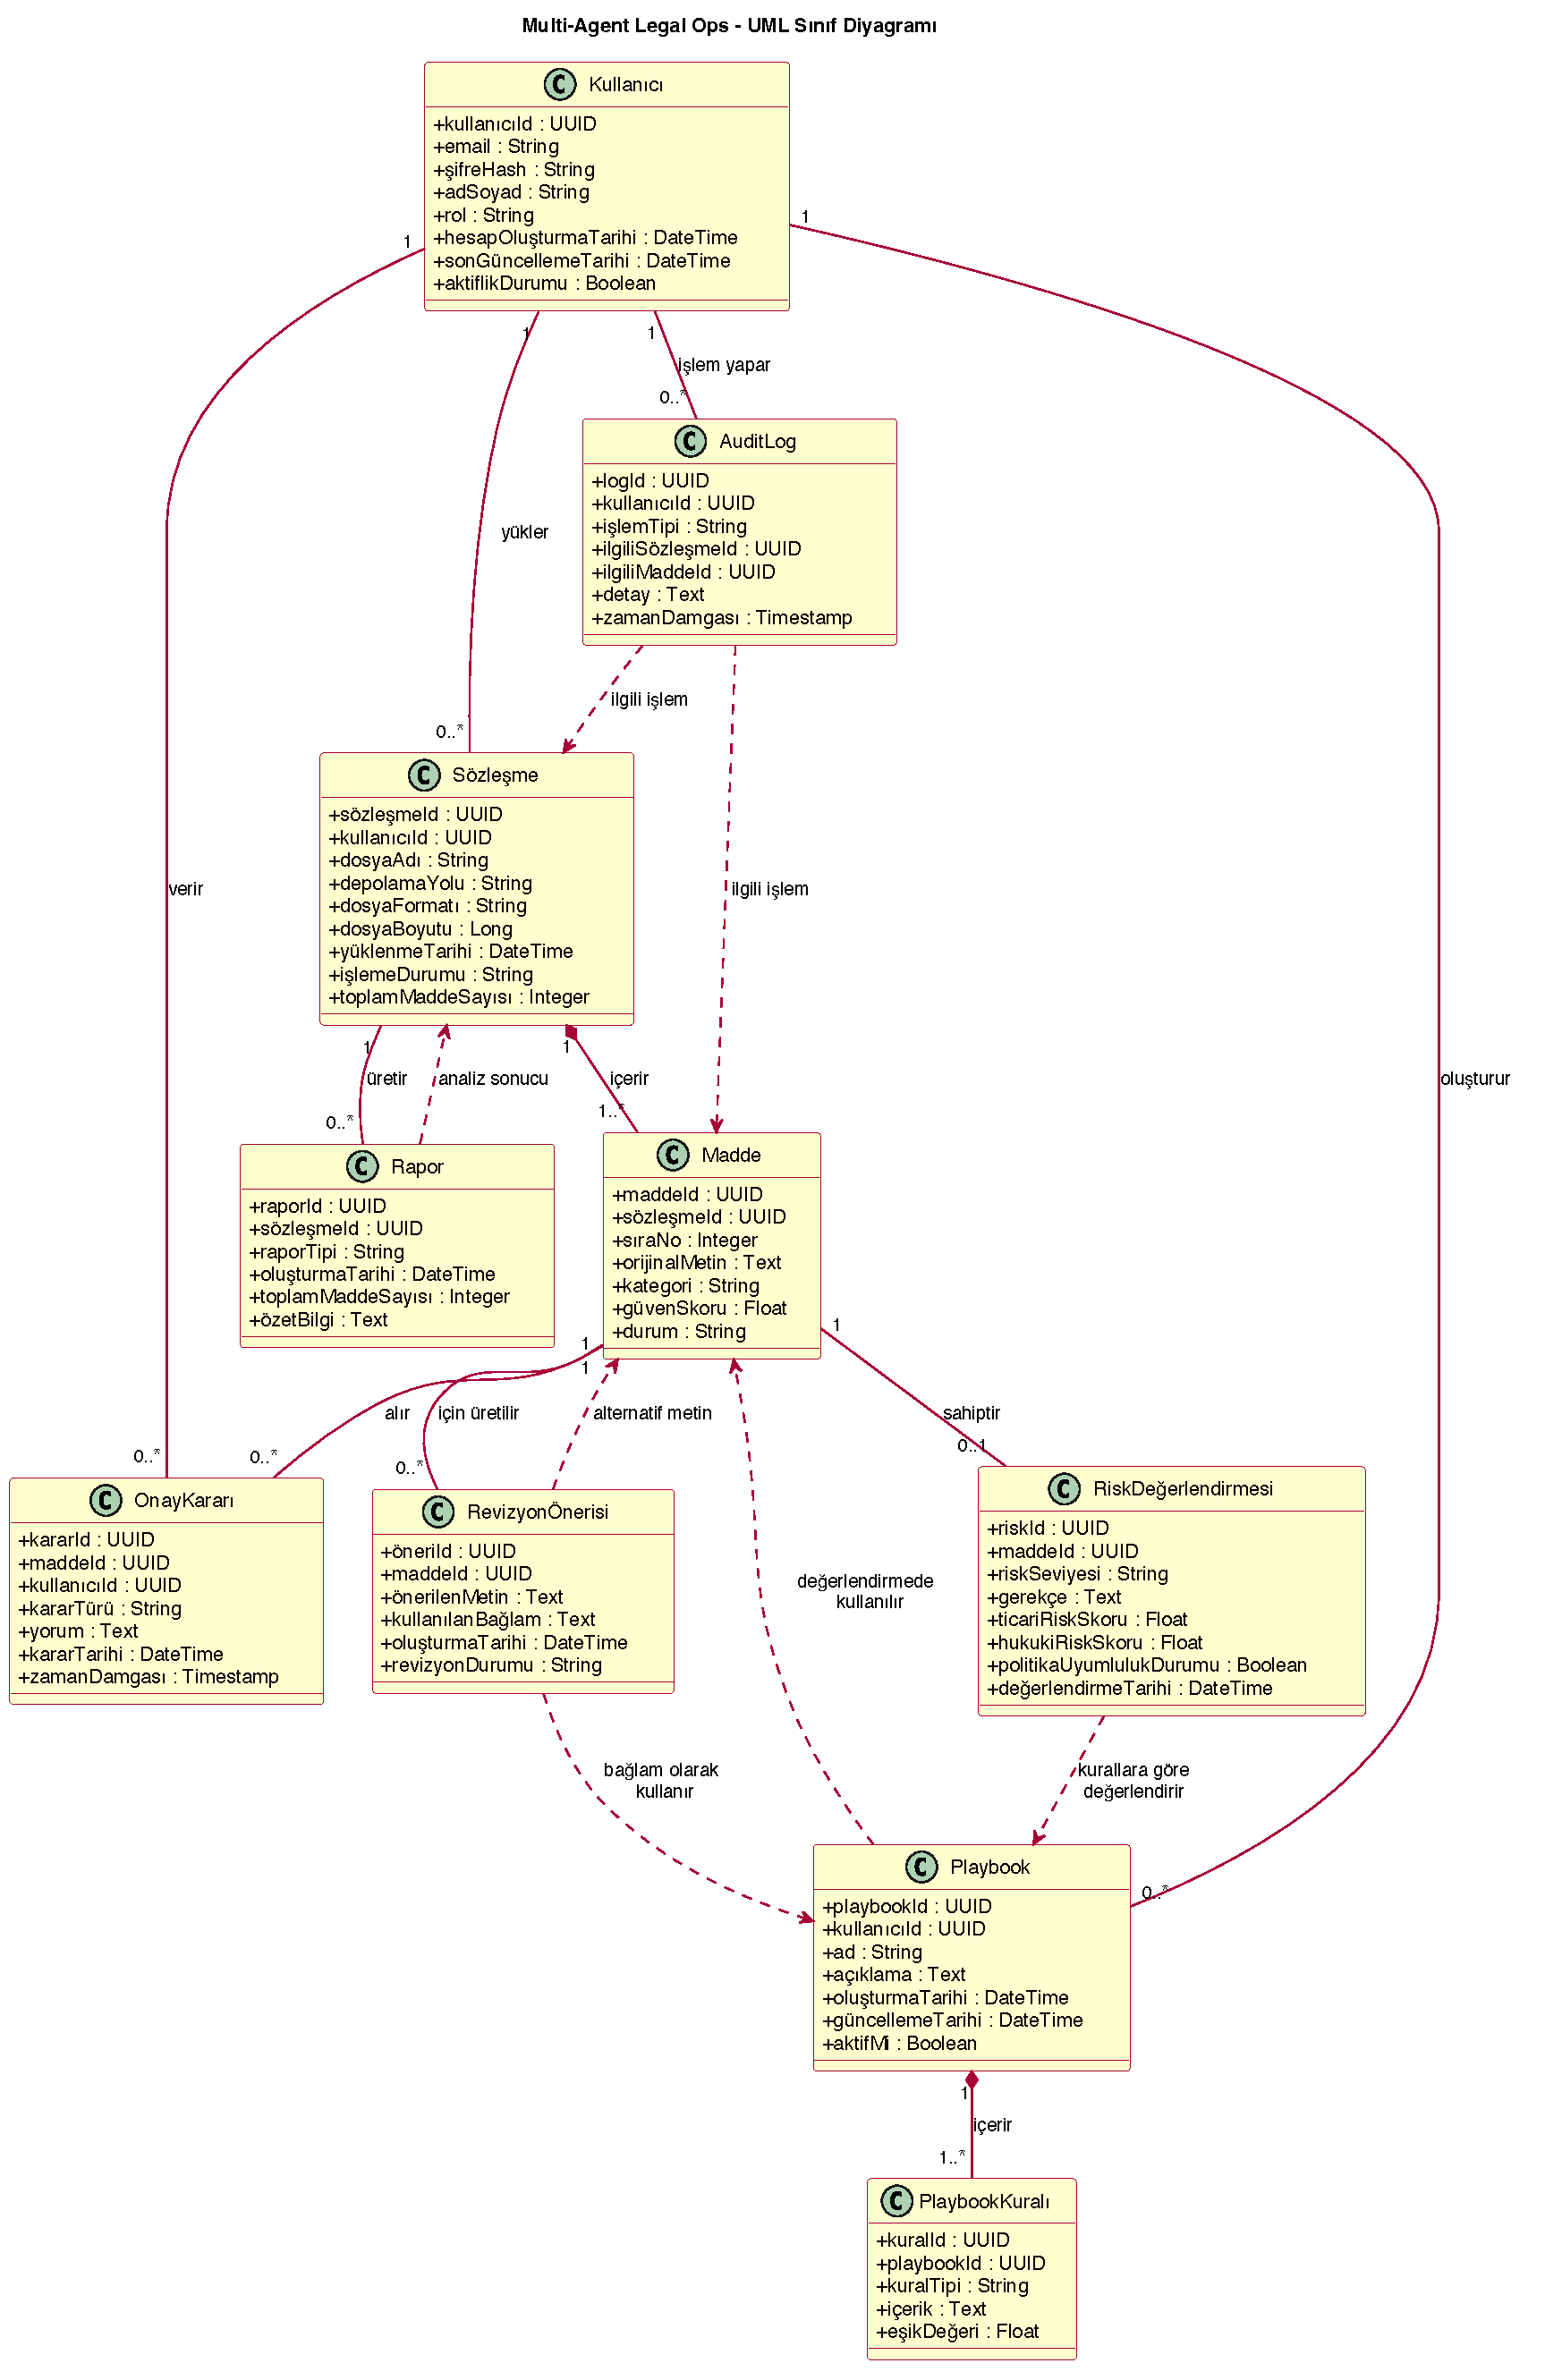
\includegraphics[height=0.85\textheight, width=0.95\linewidth, keepaspectratio]{UML.pdf}
    \captionof{figure}{Genel UML Sınıf Diyagramı}
    \label{fig:uml}
\end{minipage}

\end{landscape}

\subsection{Veri Akışı Genel Görünümü}

\subsubsection{UML Sınıf Diyagramı}
Şekil~\ref{fig:uml}, sistemin nesne yönelimli analiz kapsamındaki genel UML sınıf diyagramını göstermektedir.

\subsubsection{Veri Akışı}
Sistemdeki temel veri akışı aşağıdaki sırayı takip etmektedir:

\begin{enumerate}[leftmargin=2cm]
    \item Kullanıcı, sözleşme dosyasını web arayüzü üzerinden yükler.
    \item Doküman işleme katmanı, yüklenen dosyayı düz metne dönüştürür (gerektiğinde OCR uygular).
    \item Ayrıştırma ajanı, metni bağımsız sözleşme maddelerine böler ve her maddeyi hukuki kategorilere sınıflandırır.
    \item Risk değerlendirme ajanı, sınıflandırılmış maddeleri kullanıcı Playbook'u ve referans madde havuzu ile karşılaştırarak risk analizi yapar.
    \item Riskli bulunan maddeler için müzakere ajanı, bağlam bilgisini kullanarak alternatif ifade önerileri üretir.
    \item Tüm analiz sonuçları (sınıflandırma, risk skoru, revizyon önerisi) kullanıcıya kontrol paneli üzerinden sunulur.
    \item Kullanıcı, her madde için onay, red veya yeniden revize kararını verir.
    \item Kararlar ve ilişkili yorum bilgileri denetim izi olarak veritabanına kaydedilir.
    \item Kullanıcı isteğine bağlı olarak özet/detaylı rapor veya revize edilmiş sözleşme taslağı oluşturularak dışa aktarılır.
\end{enumerate}


\subsection{Sözlük}

\begin{longtable}{|p{4.5cm}|p{9cm}|}
\hline
\textbf{Terim} & \textbf{Tanım} \\
\hline
\endfirsthead
\hline
\textbf{Terim} & \textbf{Tanım} \\
\hline
\endhead
YKE (Yazılım Konfigürasyon Elemanı) & Yazılım sisteminin bağımsız olarak tanımlanabilen, yönetilebilen ve kontrol edilebilen bir bileşeni. Bu projede sistemin tamamını ifade eder. \\
\hline
SRS & Yazılım Gereksinimleri Belirtimi (Software Requirements Specification). Sistemin işlevsel ve işlevsel olmayan gereksinimlerini tanımlayan doküman. \\
\hline
SDD & Yazılım Tasarım Dokümanı (Software Design Document). Sistemin nasıl tasarlanacağını ve uygulanacağını tanımlayan doküman. \\
\hline
LLM & Büyük Dil Modeli (Large Language Model). Doğal dil işleme görevlerinde kullanılan yapay zeka modeli. \\
\hline
RAG & Retrieval-Augmented Generation. Bilgi erişimi ile metin üretimini birleştiren yapay zeka tekniği. \\
\hline
OCR & Optik Karakter Tanıma (Optical Character Recognition). Görüntülerdeki metni dijital metne dönüştürme teknolojisi. \\
\hline
Playbook & Kullanıcının sözleşme inceleme sürecinde kullanılmak üzere tanımladığı politikalar, kurallar ve eşik değerler kümesi. \\
\hline
Ajan (Agent) & Belirli bir görev alanında (ayrıştırma, sınıflandırma, risk analizi, müzakere) bağımsız çalışan yapay zeka bileşeni. \\
\hline
Orkestratör & Birden fazla ajanın koordineli çalışmasını sağlayan, görev dağıtımı ve sonuç toplama işlemlerini yöneten mekanizma. \\
\hline
Redline & Orijinal metin ile önerilen revizyon metni arasındaki farkları görsel olarak gösteren karşılaştırmalı görünüm. \\
\hline
Embedding & Metin verilerinin, anlamsal benzerlik araması yapılabilecek sayısal vektör temsillerine dönüştürülmesi. \\
\hline
CI/CD & Sürekli Entegrasyon / Sürekli Dağıtım (Continuous Integration / Continuous Deployment). Otomatik derleme, test ve dağıtım süreçleri. \\
\hline
Audit Trail & Denetim İzi. Sistemde gerçekleştirilen tüm kritik işlemlerin kaydını tutan günlük mekanizması. \\
\hline
API & Uygulama Programlama Arayüzü (Application Programming Interface). Yazılım bileşenleri arasındaki iletişimi sağlayan arayüz. \\
\hline
REST & Temsili Durum Transferi (Representational State Transfer). Web servisleri için kullanılan mimari yaklaşım. \\
\hline
WebSocket & İstemci ile sunucu arasında çift yönlü, gerçek zamanlı iletişim sağlayan protokol. \\
\hline
KOBİ & Küçük ve Orta Büyüklükteki İşletme. \\
\hline
\end{longtable}


\end{document}
